\documentclass[a4paper, oneside]{book}
\usepackage[utf8]{inputenc}
\usepackage[a4paper,top=2.5cm,bottom=2.5cm,left=2cm,right=2cm]{geometry}
\usepackage{amssymb}
\usepackage{amsthm}
\usepackage{graphics}
\usepackage{amsfonts}
\usepackage{amsmath}
\usepackage{amstext}
\usepackage{engrec}
\usepackage{rotating}
\usepackage[safe,extra]{tipa}
\usepackage{multirow}
\usepackage{hyperref}
\usepackage{enumerate}
\usepackage{braket}
\usepackage{marginnote}
\usepackage{pgfplots}
\usepackage{cancel}
\usepackage{polynom}
\usepackage{booktabs}
\usepackage{enumitem}
\usepackage{algorithm}
\usepackage{algpseudocode}
\usepackage{multicol}
\usepackage{framed}
\usepackage{pdfpages}
\usepackage{pgfplots}
\usepackage{fancyhdr}
\usepackage{caption}
\usepackage{subcaption}
\usepackage{setspace}
\usepackage{hyperref}

\DeclareMathOperator*{\argmax}{arg\,max}
\DeclareMathOperator*{\argmin}{arg\,min}

\pagestyle{fancy}
\fancyhead[L,RO]{\slshape \rightmark}
\fancyfoot[C]{\thepage}

\title{Advanced Machine Learning}
\author{Tommaso Ferrario (\href{https://github.com/TommasoFerrario18}{@TommasoFerrario18}) \\\\
Telemaco Terzi (\href{https://github.com/Tezze2001}{@Tezze2001})}
\date{Ottobre 2024}

\pgfplotsset{compat=1.13}

\begin{document}

\maketitle
\newtheorem{teorema}{Teorema}
\newtheorem{dimostrazione}{Dimostrazione}
\newtheorem{definition}{Definition}
\newtheorem{esempio}{Example}
\newtheorem{osservazione}{Osservazione}
\newtheorem{note}{Note}
\newtheorem{corollario}{Corollario}
\tableofcontents
\renewcommand{\chaptermark}[1]{
    \markboth{\chaptername
        \ \thechapter.\ #1}{}}
\renewcommand{\sectionmark}[1]{\markright{\thesection.\ #1}}

\chapter*{Introduction}
\textbf{Deep Learning} is a subset of machine learning that is concerned with 
neural networks that are use to learn underlying features in data.

In general, we can define machine learning as a program that starting from the 
input and the output of a system, learns the rules that govern the system. In 
order to obtain high performance, machine learning algorithms depends heavily on 
the \textbf{representation} of the data. Representation is therefore the fundamental, 
and many artificial intelligence tasks can be solved by designing the right set of features.

The most difference between Deep ML and ML is that, the first one try to learn an
efficient representation of data and than use it to train a learn model. The latter 
one use a representation of data specified by an expert to train a learn model.

Deep Learning use neural networks with many layers of activity vectors as 
representations and learning the connection strengths between that give rise to 
these vectors by following the stochastic gradient of an objective function that
measures how well the network is performing.

So, the key ingredient of deep learning is \textbf{Depth}. There are two main 
ways to measure the depth of a model:
\begin{enumerate}
    \item in terms of depth of the graph describing how concepts are related to
        each other.
    \item in terms of number of sequential instructions that must be executed to 
        evaluate the architecture. This can be influenced by the choice of basic 
        functions used.
\end{enumerate}

One solution to the problem of feature representation is to use machine learning
not only to find the mapping between input and output, but also to find the
representation itself. This approach is called \textbf{Representation Learning}.
The goal of this task is to identify the \textit{factor of variations} that 
explain the observed data. The goal of this task is to identify the factor of 
variations that explain the observed data.

The most common example of representation learning is the use of autoencoders.

A key part of representation learning consists in the \textbf{distributed 
    representation}, which means a many to many relationship between two types
of representation:
\begin{itemize}
    \item Each concept is represented by many neurons.
    \item Each neuron participates in the representation of many concepts.
\end{itemize}

Deep learning solves this central problem in representation learning by introducing
representations that are expressed in therms of other, simpler representations.
An example is bunch of letters form words, sets of words form phrases.

\chapter{Feed Forward Neural Network}
\section{Introduction}
The \textbf{Feed Forward Neural Network} (FFNN) is a particular type of neural
network where each layer is connected to the next one without loop. We can think
at each layer as a vector to a vector function.

Each layer is composed by a set of neurons, where each neuron receives a set of input
from many others, unit and computes its own activation rule.

We can think at a FFNN as a composition of many functions, where each function is
a layer. For example: if a FFNN try to approximate a function $f(x)$ and has $3$
hidden layer, we can represent it as:
\begin{equation*}
    f(x) = f^3(f^2(f^1(x)))
\end{equation*}
where $f^i$ is a function of $i$-layer. The overall length of hidden layers is
the \textbf{depth} of the model.

During the training process we want to learn a function $f(x)$ that, starting from
the training data, try to approximate the \textbf{target function} $f^*(x)$.

In the case of supervised problems, each instance $x$ is associated with a label
$y\sim f^*(x)$, therefore, the output layer at each point $x$ must produce a value
that is close to $y$.
\begin{note}
    It's important that is $y \sim f^*(x)$ and not $y=f^*(x)$ because we want a
    model that generalizes.
\end{note}

The behavior of the intermediate layers (\textbf{hidden layers}) are not directly
specified by the training data, but is the learning algorithm that must decide
how to use these layers to best implement an approximation of $f^*$. The dimensionality
of the hidden layers is called \textbf{width} of the model.

\subsection{Initialization}
Another important step inside the planning of a deep neural network is the
initialization process. Proper initialization of weights and biases is crucial
to ensure stable training and prevent issues like exploding or vanishing gradients.

First of all we can initialize all \textbf{bias} to $0$ to discover eventually
dead neurons.

For \textbf{weights} we must not initialize to the same values because we have to
brake the symmetry of the model, so we can sample weights from a normal
distribution with mean $0$ and variance dependant of the number of neurons in
the previous layer.
\begin{equation*}
    W^{[l]} \sim \mathcal{N}\left(0, \frac{1}{n^{[l-1]}}\right)
\end{equation*}
Effective initialization ensures that the gradients propagate correctly,
facilitating faster convergence during training.

\subsection{Training process}
The training process can be summarized as follows: initially, the network's weights
are randomly initialized. Then, for each training example $(x, y)$, the network
computes $f^\ast(x)$. Next the error $E(y, f^*(x))$ is calculated, and all weights
are adjusted using the gradient approximate, which is calculated with \textbf{backpropagation}.

\begin{note}
    During the training phase, the weights are adjusted every $n$ examples,
    where $n$ is the batch size. Weights are usually fixed by considering the
    elements of a batch to avoid overfitting.
\end{note}
\section{Weight Learning}
If $f(x)$ is a \textbf{non-linear} function, we can theoretically approximate it
using a hidden layer. The challenge lies in finding the right weights.

The essence of supervised machine learning is the creation of functions that can
analyze examples (instances) and produce generalizations (predict unseen data).
This involves searching over all possible functions, a task that is inherently
complex. To make this manageable, we typically restrict the set of all possible
functions to specific families, referred to as \textbf{hypothesis classes}.

One strategy to solve non-linear problem using a linear model is to use a
transformation of the input space. By modifying the data representation, we can
apply \textbf{non-linear transformation} ($\phi$) to the inputs. In other words,
given an instance $x$, $\phi(x)$ represents a new set of features describing $x$.

There are several way to define a transformation:
\begin{itemize}
    \item Use a predefine $\phi$ called \textbf{kernel}
    \item Define manually $\phi$ but it isn't convenient.
    \item We can learn it but it isn't a general transformation. This is the
          approach used by deep learning.
\end{itemize}

In deep learning the goal is to learn the transformation $\phi$, whereas SVM use
a predefine \textit{kernel}. So, we can describe this approach using the
following model:
\begin{equation}
    f(x, \theta, \omega) = \phi(x; \theta)^T \cdot \omega
\end{equation}
Here, $\theta$ represents the parameters used to learn the transformation $\phi$
from a broad class of functions, while $\omega$ represents the parameters mapping
$\phi(x)$ to the target.

\begin{note}
    In a deep learning model, $\phi$ defines a hidden layer.
\end{note}

The prediction model is typically a high dimensional linear function, $f(x): x \cdot W + b$
which is combine with a non-linear function $\sigma$ to produce the output of the
model. Below are some examples:
\begin{itemize}
    \item \textbf{Sign function}: this function is used for binary classification:
          \begin{equation}
              \hat{y} = sign(f(x))
          \end{equation}
    \item \textbf{Sigmoid function}: Used for binary classification when confidence
          in decisions is required, such as in log-linear binary classification:
          \begin{equation}
              \hat{y} = \frac{1}{1+e^{-f(x)}}
          \end{equation}
    \item \textbf{Softmax}: this is used for multi-class classification, suppose
          to have $k$ classes:
          \begin{equation}
              \hat{y} = softmax(f'(x)) = \frac{e^{f'(x)_i}}{\sum_{j=1}^k e^{f'(x)_j}}
          \end{equation}
\end{itemize}

\textbf{Pros} for linear models are that can be fit efficiently and reliably, because
gradient on linear model are easy to compute.

\textbf{Cons} models are restricted to linear functions so they works for data linear
separable, solved by a transformation.
\subsection{Kernel trick}
Transform the input space into an higher-dimensional space can be useful to solve
non-linear separable problem. However, this approach increase the number of
parameters and the complexity of the model. To address this challenge, we can map
the input space into a higher-dimensional space using specific functions called
\textbf{kernels}.

\begin{note}
    There can be many transformations that allow the data to be linearly separated
    in higher dimensions, but not all of these functions qualify as kernels.
\end{note}

This approach is functional because we can use the \textbf{kernel trick} to operate
in the original feature space without computing the coordinates of the data in a
higher-dimensional space.

A general linear model would be rewritten as:
\begin{equation}
    \omega^T x + b = b+ \sum_{i=1}^m \alpha_ix^Tx^{(i)}
\end{equation}
where $b$ is the bayes, $\alpha_i$ is a coefficient, $x$ is a point, $x^{(i)}$ is
$i$-th instance of training set and $m$ is the number of training instances.

To apply this model on non-linear separable data, we introduce a transformations
$\phi$ to the input space, resulting in:
\begin{equation}
    f(x) = \omega^T \cdot x + b = b + \sum_{i = 1}^m \alpha_ix^Tx^{(i)} = b +
    \sum_{i=1}^m \alpha_i\phi (x^T) \cdot \phi(x^{(i)})
\end{equation}
The kernel trick override $\phi(x^T) \cdot \phi(x^{(i)})$ with $k(x^T, x^{(i)})$,
where $k(\cdot , \cdot)$ is the kernel function. This eliminates the need to
compute $\phi(x)$ directly, making it computationally more efficient.

Furthermore, kernel trick allows us to learn models that are non-linear functions
of $x$ using a convex optimization techniques, which are guaranteed to converge
efficiently. This is possible because $\phi $ is fixed, and we optimize only the
coefficient $\alpha_i$. In Support Vector Machines (SVMs), only support vectors
are used in the model, and $\alpha_i= 0$ if and only if $i$ is not a support vector.

Any algorithm that uses kernel is called \textbf{kernel machines} or \textbf{kernel
    methods}

\section{Loss/Cost function}
\begin{definition}[\textbf{Loss function}]
    A \textbf{loss function} maps the outcome of a single data point, represented
    by one or more variables, to a real number. This number intuitively reflects
    the network's performance on that specific data point.
\end{definition}
\begin{definition}[\textbf{Cost function}]
    A \textbf{cost function} maps the average loss over an entire dataset to a
    real number, representing the overall performance of the model.

    A cost function should align with the intended purpose of the network to
    ensure effective optimization.
\end{definition}
With these definitions, we can state that the goal of a training algorithm is to
minimize the cost function. Lower values of the cost function generally indicate
better network performance.

There is a wide range of loss functions that can be used in deep learning, so we
need to choose the right one for our problem. The choice of a loss function depends
on the specific task the model is intended to solve. Below are common examples of
loss functions for classification and regression tasks.
\paragraph{Classification loss functions}
\begin{itemize}
    \item \textbf{Maximum likelihood}: this approach optimizes the likelihood of
          the model's predictions matching the target distribution:
          \begin{equation}
              \mathcal{L} = - \frac{1}{N} \sum_{i=1}^N y_i p(\hat{y}_i) +
              (1-y_i) p(1-\hat{y}_i)
          \end{equation}
    \item \textbf{Binary Cross-entropy (log-loss)}: Used for binary classification tasks:
          \begin{equation}
              \mathcal{L} = - \frac{1}{N} \sum_{i=1}^N y_i \log(p(\hat{y}_i))
              + (1-y_i) \log(p(1-\hat{y}_i))
          \end{equation}
    \item \textbf{Categorical Cross-entropy}: Suitable for multi-class classification problems:
          \begin{equation}
              \mathcal{L} = - \sum_{i=1}^N y_i \log(p(\hat{y}_{i}))
          \end{equation}
\end{itemize}
\paragraph{Regression loss functions}
\begin{itemize}
    \item \textbf{Mean Squared Error}: Measures the average squared difference
          between the predicted and actual values:
          \begin{equation}
              \mathcal{L} = \frac{1}{N} \sum_{i=1}^N (y_i - \hat{y}_i)^2
          \end{equation}
    \item \textbf{Mean Absolute Error}: Measures the average absolute difference
          between predictions and targets:
          \begin{equation}
              \mathcal{L} = \frac{1}{N} \sum_{i=1}^N |y_i - \hat{y}_i|
          \end{equation}
    \item \textbf{Huber Loss}: Combines the properties of MSE and MAE to handle
          outliers effectively:
          \begin{equation}
              \mathcal{L} = \frac{1}{N} \sum_{i=1}^N \begin{cases}
                  \frac{1}{2}(y_i - \hat{y}_i)^2                  & \text{if } |y_i - \hat{y}_i| \leq \delta \\
                  \delta |y_i - \hat{y}_i| - \frac{1}{2} \delta^2 & \text{otherwise}
              \end{cases}
          \end{equation}
\end{itemize}
\begin{note}
    The list above is not exhaustive; many other loss functions exist for specialized
    tasks.

    It is possible to define custom loss functions. In such cases, it is crucial
    that the function is differentiable, as this ensures compatibility with
    gradient-based optimization methods.
\end{note}
\section{Gradient optimization}
Since the goal of our network is to approximate a target function, we need to
measure the difference between the predicted function, that we have learned, and
the target function using a \textbf{loss function}.

Formally, this function $\mathcal{L}(\hat{y}, y)$ return a scalar value that
quantifies how well the prediction $\hat{y}$ matches the target $y$. To minimize
the optimization problem over training sample, we include the parameters of the
model $\theta$ to the loss function:
\begin{equation}
    J(\theta) = \frac{1}{n} \sum_{i=1}^n \mathcal{L}(x_i; y_i; \theta)
\end{equation}
where $n$ is the number of training samples.

The main objective of the training algorithm is to find the optimal set of
parameters $\theta$ that minimize the loss function. Formally, this can be written
as:
\begin{equation}
    \hat{\theta} = \argmin_{\theta} J(\theta) = \argmin_{\theta} \frac{1}{n}
    \sum_{i=1}^n \mathcal{L}(x_i; y_i; \theta)
\end{equation}

In deep learning, we aim to minimize the \textbf{loss function}, which, in the
context of optimization, is referred to as the \textbf{objective function}. To
achieve this, we use partial derivatives $\frac{\delta}{\delta x_i} f(x)$ to
measure how the loss function changes when only the variable $x_i$ is varied.

The \textbf{gradient} $\nabla f(x)$ generalizes the concept of derivative to
higher dimensions. In other word, the gradient is a vector where the $i$-th element
represents the partial derivative of the function with respect to $x_i$.

To minimize the loss function, we move in the direction opposite to the gradient.
This approach, known as \textbf{gradient descent}, is defined as:
\begin{equation}
    x' = x - \eta \nabla f(x)
\end{equation}
where $x$ is the current point, $x'$ is the updated point, $\eta$ is the learning
rate and $\nabla f(x)$ is the gradient of the loss function.

\begin{note}
    The gradient descent converge when every element of the gradient is zero.
\end{note}

The \textbf{learning rete} is an hyperparameter that controls the step size in
the gradient's direction. The optimal value of $\eta$ may change during the training,
but do to computational cost, it is often kept fixed. A good strategy involves
starting with a high learning rate to explore different paths and reduce the
likelihood of getting stuck in a local minimum, and then gradually decreasing it
to converge to the global minimum.

Since in many loss function are not convex, they cannot be optimized in a close
form. Instead, we use iterative numerical optimization method to find the minimum
of the loss function.

In some cases, evaluating the loss function directly may be computationally
expensive. However, as long as we can approximate the gradient, iterative
numerical methods can still be applied.

To reduce the risk of overfitting, a \textbf{regularization term} can be added
to the loss function:
\begin{equation}
    \hat{\theta} = \argmin_{\theta} \frac{1}{n} \sum_{i=1}^n \mathcal{L}(x_i; y_i; \theta)
    + \lambda R(\theta)
\end{equation}
where $\lambda$ is an hyperparameter that balances the trade-off between bias and
variance, and $R(\theta)$ is the \textbf{regularization term}, a scalar that
reflecting the model complexity. The regularization term discourages the model from
fitting the noise in the training data. This term does not always appear in the
loss function, but we can apply it implicitly by changing the network architecture
or altering the data. Examples of these operations are:
\begin{itemize}
    \item Disable some connections in the network.
    \item Add noise to the input data.
\end{itemize}
\begin{note}
    Networks with smaller weights tend to generalize better than those with larger
    weights. This is because noise in the input data has a more significant impact
    on networks with large weights.
\end{note}
\subsection{Stochastic Gradient Descent}
The \textbf{Stochastic Gradient Descent} (SGD) is a variant of the gradient descent
algorithm that is used to train neural networks. The computational cost of computing
the gradient of the loss function for the entire training dataset is $\mathcal{O}(n)$,
where $n$ is the number of training examples. To reduce this cost, SGD approximates
the gradient by computing it on a subset of the training data.

In its simplest form, SGD updates the model parameters after computing the gradient
on a single training example (known as \textbf{Online Learning}). While this approach
can lead to faster updates, it often results in slow convergence and noisy gradients.

To address these issues, a \textbf{mini-batch} approach is commonly used. A mini-batch
is a small, randomly selected subset of the training data, typically ranging from
1 to a few hundred examples. By computing the gradient on a mini-batch, the
algorithm achieves a balance between convergence stability and computational
efficiency.

We can compute the gradient of the loss function on the mini-batch as follows:
\begin{equation}
    g = \frac{1}{m} \sum_{i = 1}^{m} \nabla_{\theta} \mathcal{L}(x_i, y_i, \theta)
\end{equation}
where $m$ is the size of the mini-batch, $x_i$ and $y_i$ are the predicted
and actual labels for the $i$-th training example, respectively, and $\nabla_{\theta}
    \mathcal{L}(x_i, y_i, \theta)$ is the gradient of the loss function with
respect to the model parameters $\theta$.

The model parameters are then updated as follows:
\begin{equation}
    \theta = \theta - \eta g
\end{equation}
where $\eta$ is the learning rate, and $g$ is the gradient computed on the mini-batch.

When we choose the mini-batch size, we have to consider the trade-off between
the computational efficiency and the convergence speed. In general, the larger
the mini-batch size, the more accurate the estimate of the gradient, but the
slower the convergence. While the smaller the mini-batch size, the noisier the
estimate of the gradient, but the faster the convergence.
\section{Output function}
The choice of the loss function is closely related to the choice of the \textbf{
    output unit}, which is the final layer of a neural network. The output unit
is responsible for transforming the features generated by the network into the
appropriate format for the task at hand.

There are many output units that can be used in deep learning, here are some examples:
Linear, Sigmoid, Softmax, Gaussian Mixtures.
\subsection{Linear output unit}
One simple output unit is the linear unit, which is based on linear model:
\begin{equation}
    \hat{y} = W^T \cdot h + b
\end{equation}
where $W$ and $b$ are the learnable weights and bias, and $h$ represents the features
from the previous layer.

Linear output units are typically used in regression tasks where the target variable
can take any real value. They are also used for modeling the mean of a Gaussian
distribution. However, they are unsuitable for classification problems, as they
do not constrain the output to a specific range, such as probabilities.
\subsection{Sigmoid output unit}
The sigmoid output unit is used for binary classification task. The output
of this unit is a value between $0$ and $1$ and it can be interpreted as the
probability of the input belonging to the positive class.

This function can be approximated using the linear output unit, but the function
we create would have 0 gradient outside the $[0, 1]$ range, so the learning
algorithm would not be able to update the weights.

The sigmoid function resolve the previous problem, because it ensure a strong
gradient whenever the model has a wrong answer. The sigmoid function is defined as:
\begin{equation}
    \sigma(x) = \frac{1}{1+e^{-x}}
\end{equation}
\subsection{Softmax output unit}
The softmax output unit is used for multi-class classification tasks. It produces
a probability distribution over $k$ classes, where each value indicates the likelihood
of the input belonging to a specific class. To implement this we need to have a
linear layer to predicts the un-normalized log probabilities and then we apply
the softmax function to normalize the output.

The softmax function is defined as:
\begin{equation}
    \sigma(x)_i = \frac{e^{x_i}}{\sum_{j=1}^k e^{x_j}}
\end{equation}
where $x_i$ is the unnormalized log probability for the $i$-th class.

The softmax function is a good output function because is continuous and
differentiable.

It preserves the relative order of the input values, ensuring that the class with
the highest log probability remains the most likely after normalization.

The output of the softmax function can be interpreted as the probability of the
input belonging to each class. However, the model may overfit to known classes,
potentially misclassifying inputs from unknown or unseen classes with high confidence.
\subsection{Gaussian Mixtures output unit}
In some cases, we need to perform multimodal regression, where the target variable
$y$ is drawn from a conditional distribution $p(y|x)$ that exhibits multiple peaks
for the same input $x$.

To model such distributions, we can use a \textbf{Gaussian Mixture Model} (GMM),
defined as:
\begin{equation}
    p(y|x) = \sum_{i=1}^n p(c= i|x) N(y; \mu^{(i)}(x), \Sigma^{(i)}(x))
\end{equation}
where the Neural network output have the following value:
\begin{itemize}
    \item $p(c=i|x)$ is the mixture component, representing the probability of
          selecting the $i$-th Gaussian.
    \item $\mu^{(i)}(x)$ is the mean of the $i$-th component.
    \item $\Sigma^{(i)}(x)$ is the covariance matrix of the $i$-th component.
\end{itemize}
\section{Activation Function}
A \textbf{hidden unit} applies an affine transformation to its inputs, defined as:
\begin{equation}
    z = Wx + b
\end{equation}
where $W$ is the weight matrix, $x$ is the input vector and $b$ is the bias vector.

The result of this transformation is passed through a \textbf{non-linear function}
called the \textbf{activation function}. The choice of activation function
significantly impacts the network's ability to learn complex patterns.

\subsection{Tanh}
The \textbf{tanh} function is similar to the sigmoid function but maps negative
inputs to strongly negative values, and zero inputs to zero, making it centered
at zero.

Some important characteristics are that the $\tanh$ is \textbf{differentiable}
and \textbf{monotonic}, but its derivative isn't \textbf{monotonic}.
\begin{note}
    The $\tanh$ function is used for \textbf{binary classification} problems.
\end{note}

The $\tanh$ function has larger derivatives compared to the sigmoid function,
which can help accelerate training by reducing the vanishing gradient problem.
\subsection{Rectified Linear Unit}
The \textbf{Rectified Linear Unit} (ReLU) is the most used activation function
in neural networks. It is described as:
\begin{equation}
    g(x) = \max[0,z]
\end{equation}
ReLU introduces sparsity by deactivating neurons for negative inputs (outputting
0). Although it is non-differentiable at $z = 0$, this rarely poses practical
problems since gradient-based methods approximate the derivative.

ReLU allows us to simplify the model because we can get a sparse representation
of the network, due the possibility to deactivate some neurons. This is possible
thanks to negative input which will be converted to zero so it will be deactivated.

Since ReLU have a ``problem'' with the $0$ value, there are some generalization
that can be used to solve this. In order to do this, we can express the ReLU as
a generalization of the following formula:
\begin{equation}
    h_i = g_i(z,\alpha) = max(0,z_i) + \alpha_i min(0, z_i)
\end{equation}
Other versions of ReLUs are:
\begin{itemize}
    \item \textbf{Absolute value rectification}: this function is obtained by
          fixing $\alpha_i = -1$ to express $g(z) = |z|$. It is used to object
          recognition.
    \item \textbf{Leaky ReLU}: this function is obtained by fixing $\alpha_i = 0.01$.
          This one solves the problem of zero gradient which means that the model
          doesn't learn. This is done by Leaky ReLU with a small linear component
          for negative input.
    \item \textbf{Parametric ReLU}: this function is like Leaky ReLU but the
          parameter $\alpha_i$ is learned.
    \item \textbf{Maxout units}: the activation function $f$ is learned. It
          combines different ReLU to produce a convex function. (Figure \ref{fig:Maxout})
          \begin{figure}[!ht]
              \centering
              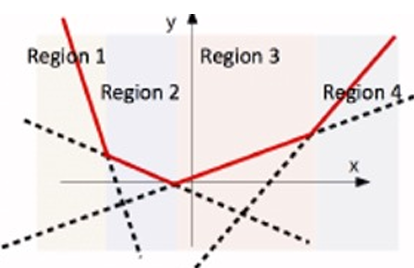
\includegraphics[width=0.5\textwidth]{img/maxout.png}
              \caption{Maxout units}
              \label{fig:Maxout}
          \end{figure}
    \item The \textbf{Softplus} function is a smooth approximation of ReLU, defined as:
          \begin{equation}
              f(x) = \log(1+e^x)
          \end{equation}
          This function was defined to solve ReLU's problem of non differentiable
          point, it is a smooth approximation of ReLU. Theoretically we can think
          to get better performance using this function compared to ReLU. However,
          empirical studies show that ReLU often outperforms Softplus in practice,
          despite its theoretical advantages.
\end{itemize}
\subsection{Guidelines for choosing activation functions}
There are some guides to use these activation functions:
\begin{itemize}
    \item Sigmoids and their combinations generally works better in case of classifiers.
    \item Sigmoids and tanh sometimes are avoided due the vanishing gradient problem.
    \item ReLU is the default activation function for hidden layers.
    \item We can use Leaky ReLU if we encounter a case of dead neurons.
    \item ReLU should only be used for hidden layer.
\end{itemize}
In general we can initially use ReLU, than if we cannot obtain better performance
we can change activation function.
\section{Regularization}
\textbf{Regularization} is a crucial technique in deep learning to prevent
\textit{overfitting}, which occurs when a model performs well on training data
but poorly on unseen data. Regularization strategies aim to reduce the model's
variance at the cost of slightly increasing its bias. This trade-off results in
a model that generalizes better to new data. Below we will list some of the
regularization techniques that we will go to see:
\begin{itemize}
    \item Parameters norm penalties;
    \item Dataset augmentation;
    \item Noise robustness;
    \item Early stopping;
    \item Parameter tying and parameter sharing;
    \item Multitask learning;
    \item Bagging and other ensemble methods;
    \item Dropout;
    \item Adversarial training;
\end{itemize}

We need to have a model that is capable to generalize on unseen data, so we have
to find the right trade-off in order to avoid overfitting and underfitting.

In the context of deep learning, most regularization strategies are based on
\textbf{regularizing estimators}. This is done through reducing \textbf{variance}
at the expense of increasing the \textbf{bias} of the estimator.
\begin{note}
    A good estimator is one that decreases the variance without increasing too
    much the bias.
\end{note}

When we are working with deep learning to solve complex tasks, we can encounter
different problems. This can increase the complexity of the model and the risk of
overfitting. In this case, we can find the best large model and in the end apply
a regularization process to reduce the complexity of the model and improve the
generalization.

The concept of regularization in machine learning and deep learning is to create
models that not only minimize the loss function but also manage the variability
and generalization capability of the model. To accomplish this, we can employ the
following strategies:
\begin{itemize}
    \item \textbf{Directly}: incorporates prior knowledge or expresses a generic
          preference for simpler models by directly altering the model or its
          training process. This is implemented by changing constraints, adding
          restrictions on the parameter values or changing objective function.
          The constraints serve to penalize certain values of the parameters;
    \item \textbf{Undirectly}: this method does not manipulate the model directly
          but alters the training process or data to enhance generalization. This
          can be done using technique such as data augmentation, introducing noise
          in the training data or using ensemble methods.
\end{itemize}
\subsection{Regularization strategies}
\subsubsection{Parameters Norm Penalties}
The most traditional form of regularization consists in adding a penalty term to
the loss function, encouraging smaller or sparser parameter values. It can be
formulated as:
\begin{equation}
    \hat{J}(\theta) = J(\theta) + \alpha \Omega(\theta)
\end{equation}
where $\alpha \in [0, \infty)$ is a hyperparameter that regulates the contribution
of the norm penalties, and $\Omega(\theta)$ is the penalty term. This parameter
can change for each layer.

Since we have added a penalty term, the optimizer will try to minimize the loss
function and at the same time it decreases some measure of the size of the
parameters $\theta$. It affects only a subset of parameters.

$\Omega$ usually penalizes only the weights ($W$) of the affine transformation
at each layer, not the bias ($b$).

This method can be implemented using different norms, here we can see some of them:
\begin{itemize}
    \item \textbf{Sum of the weights} or \textbf{$L_1$ Norm} ($L_1$): Promotes
          sparsity pushing all values to $0$ penalizing small weights more than big one.
          \begin{equation}
              \Omega(w) = \sum_{w_j}|w_j| = \|w\|_1
          \end{equation}
    \item \textbf{Sum of the squared weights} or \textbf{$L_2$ Norm} ($L_2$):
          penalizes larger weights, encouraging smoothness:
          \begin{equation}
              \Omega(w) = \sum_{w_j}|w_j|^2 = \|w\|_2
          \end{equation}
    \item \textbf{$p$-norm} ($L_p$): for $p < 2$ encourage sparser vector, while
          larger values of $p$ discourage large weights more:
          \begin{equation}
              \Omega(w) = \sqrt[p]{\sum_{w_j}|w_j|^p} = \|w\|_p
          \end{equation}
          In general, all the $p-$norms are used to penalize large weights more
          than small ones.
\end{itemize}

The effect of the $L_2$ norm is to shrinks weights on features that add noise to
the model (feature with high variance but low covariance with target), while
$L_1$ norm provides a solution that is sparse. This property can be seen as a
features selection mechanism.
\begin{note}
    Using $L_2$ negative and positive weights moves towards 0 depending on the
    magnitude of the weights, while using $L_1$ negative and positive weights
    moves towards 0 regardless of magnitude.
\end{note}

Another improve that we can add to the previous model are constraints related to
regularization term, for example, if we consider the following loss function:
\begin{equation}
    \hat{J}(\theta) = J(\theta) + \alpha \Omega(\theta)
\end{equation}
we can add a constraint to the regularization term as follows:
\begin{equation}
    \Omega(\theta) \le k
\end{equation}
where $k$ is a small value. In this way the optimization problem changed because
we have to consider also the upper-bound of regularization term.

To solve this problem, we can construct a generalize \textbf{Lagrange function},
consisting of the original objective function plus a set of penalties. Each
penalty is a product between a coefficient, called a Lagrange multiplier ($\alpha$),
and a function representing whether the constraint is satisfied.
\begin{equation}
    \mathcal{L}(\theta, \alpha; X,y) = J(w;X,y)+ \alpha(\Omega(\theta)-k)
\end{equation}
Formally the optimization problem will be:
\begin{equation}
    \argmin_\theta \max_{\alpha \geq 0} \mathcal{L}(\theta, \alpha)
\end{equation}

To solve this problem we can use techniques that minimize $J$ and then project
the solution obtained to the feasible region $\Omega(\theta) - k$. This method
prevent to get stuck in local minimum and impose stability on the optimization
procedure.
\subsubsection{Dataset augmentation}
We can get better generalization training model on more data. The main problem is
that data is limited also labelling is an extremely tedious task. \textbf{Dataset
    augmentation} provides a cheap easy way to increase the amount of your
training data.

Moreover, when you are comparing different algorithms you have to compare on
augmented and non augmented dataset to avoid bias.

To implement this technique, there are many algorithms available, but when we
use them, it's important to be cautious about introducing bias or altering the
output in the dataset.
\subsubsection{Noise robustness}
\textbf{Noise injection} can be thought of as a form of regularization. When we
add a noise with infinitesimal variance at input of the model is equivalent to
imposing a penalty on the norm of the weights.

Noise can be injected at different levels of deep models, if we add on input we
are defining a data augmentation procedure, so we have to use some of the best
practices explained before.

Adding small noise pushes model into regions where the model is insensitive to
small variations in weights, finding points that are not merely minima, but
minima surrounded by flat regions.

Since some dataset present mistake on the labels, we can remedy this problem by
adding noise to the labels. This can be done through setting a probability $\varepsilon$
for which we think the labels are correct.

This method implemented analytically in the \textbf{cross entropy} function.
Another example of this technique is \textbf{label smoothing}, where we use
softmax activation function in the output layer to get a probability.
\begin{equation*}
    \left[\begin{array}{c}
            1 \\0\\\vdots\\ 0
        \end{array}\right]_{label} \implies \left[\begin{array}{c}
            0.9 \\0.01\\\vdots\\ 0.02
        \end{array}\right]_{label}
\end{equation*}

Using a softmax we will never predict 0 or 1 but it will predict a probability so
model can always learn and make more extreme prediction forever. This has the
advantage of preventing the pursuit of hard probabilities without discouraging
correct classification.
\subsubsection{Multitasking learning}
\textbf{Multitasking learning} is a way to improve generalization by pooling the
examples arising out of several tasks. It is usually performed through the
following architecture:
\begin{itemize}
    \item \textit{Task-specific parameters}: which only benefit from the examples
          of their task to achieve good generalization.
    \item \textit{Generic parameters}: parameters shared across all tasks which
          benefit from the pooled data of all tasks.
\end{itemize}
\begin{figure}[!ht]
    \centering
    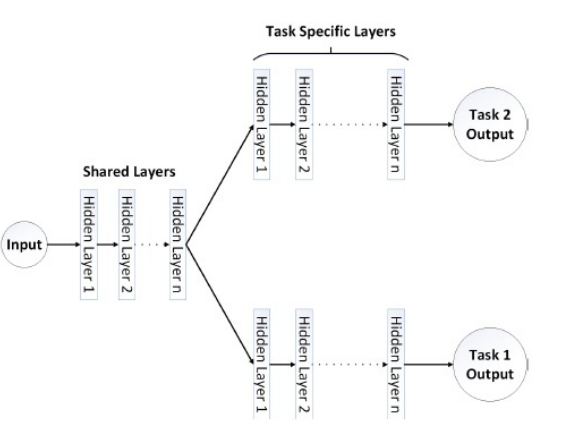
\includegraphics[width=0.5\textwidth]{img/multitask.png}
    \caption{Multitasking learning}
    \label{fig:multitask}
\end{figure}
\begin{note}
    Multitasking learning is a form of parameter sharing.
\end{note}

Shared parameters improve generalization in proportion of number of examples for
the general task. Additional task imposes constraints on the parameters in the
shared layers preventing overfitting.
\begin{note}
    Improvement in generalization only occurs when there is something shared across
    the tasks at hand.
\end{note}
\subsubsection{Early stopping}
When training large models with sufficient representational capacity to overfit
the task, we often observe that training error decreases over time but validation
error begins to rise again. We can obtain a model with better validation error by
returning to the parameter setting at the point in time with the lowest validation
error.

\textbf{Early stopping} is one of the most common techniques used. We can think
at this technique as a hyperparameter selection method, where training time is
the hyperparameter to be chosen.

Early stopping can be implemented as follow:
\begin{enumerate}
    \item Choose number of iterations $n$
    \item Train model for $n$ iterations
    \item Validate model and compute validation error, compare consecutive validation
          error and return to point 2 until delta is insignificant or negative.
\end{enumerate}
Every iteration model improves its weights until it starts to going in overfitting.
\begin{note}
    It's impossible to write all parameters on disk during training.
\end{note}
\begin{figure}[!ht]
    \centering
    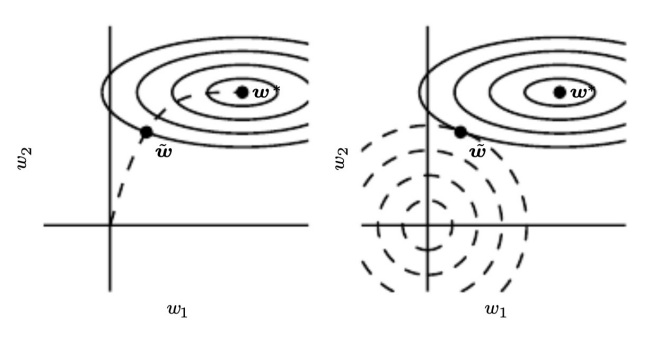
\includegraphics[width=0.5\textwidth]{img/early_stopping.png}
    \caption{On the left we can see the process of early stopping, while on the
        right we can see a classic regularization process.}
    \label{fig:earlystopping}
\end{figure}
\subsubsection{Parameters Tying}
\textbf{Parameters Tying} refers to explicitly forcing the parameters of 2 models
to be close to each other using the norm penalty:
\begin{equation}
    \|w(A)- w(b)\|
\end{equation}
with $A$ and $B$ respectively first and second model. This norm penalty is added
to the objective function like a constraint. It is used in Siamese networks,
convolution operators and multitasking learning.
\subsubsection{Bagging}
\textbf{Bagging} is a technique for reducing generalization error combining
several models (\textbf{ensemble model}).

You have to train $k$ different models on $k$ different subsets of training data
with same number of examples as original dataset using a random sampling with
replacement.

Every model is then tested, they produce $k$ votes for the final result. These
models are called ensemble.

The objective of this method is to introduce generalization by using different
models trained on different examples using different initialization hyperparameter
and different structures to have independent errors.

Cons of this method is that ensemble models doesn't provide us a scalable way to
improve performance, moreover we have 2-3 models inside the ensemble.
\subsubsection{Dropout}
\textbf{Dropout} provides a computationally inexpensive but powerful method of
regularizing a broad family of models. It provides an inexpensive approximation
of a ensemble with a high number of sub-networks of the starting one.

All the sub-networks should be formed by removing non-output units from underlying
base network, generating an exponential number of models, using a treatable
amount of memory.

This technique eliminates the need to accumulate model votes in the inference
phase. It is intended to train the model to be learned by switching on and off
with different probabilities input neurons or neurons in the hidden layers.

To do a train phase we use a \textbf{minibatch-based learning algorithm} that
makes small steps, such as stochastic gradient descent.

Each time we change minibatch we \textbf{randomly sample} a different binary mask
to apply to all input and hidden units in the network. Typically the distribution
use for sampling is not uniform. For example, the probability of keeping a hidden
unit is $0.5$, while the probability of including an input unit is $0.8$.

We can have some problem, indeed, at training time we are required to divide the
output of each unit by the probability of that unit's dropout mask, so we assign
as likelihood on the output. In this way we make sure that the expected total
input to a unit at test time is the same as the expected total input of that unit
at train time.

We haven't theoretically basis for the accuracy but empirically it perform well.
Complexity of dropout is limited to a $\mathcal{O}(n)$ computation per example
to update because it needs to generate a total of $n$ random numbers and multiply
them by the state.

Dropout can be used with every model and also with stochastic gradient descent.
The cost of applying dropout to the entire model could be significant, but the
amount of benefit on generalization error couldn't be enough to the cost of the
regularization.
\subsubsection{Adversarial training}
We can add \textbf{adversarial examples} (inputs perturbed by noise) to train the
model for robustness. These are used to train the network and will allowed us to
reduce test errors.

Adversarial examples can be generated by adding to a bit of perturbation on some
train example with a low multiplication factor of noise. This method allowed us
to generate new examples for training from the original train set with slightly
changes that are unrecognized by humans.
\section{Generative Adversarial Models}
\textbf{Generative Adversarial Network} (GAN) are generative model that
implicitly learn the \textbf{data distribution} from a zero-sum game between 2
computing neural network:
\begin{itemize}
    \item \textbf{Discriminator}: a neural network that classify examples between
          fake and real.
    \item \textbf{Generator}: generate fake example that are given as input to the
          discriminator.
\end{itemize}

\begin{figure}[!ht]
    \centering
    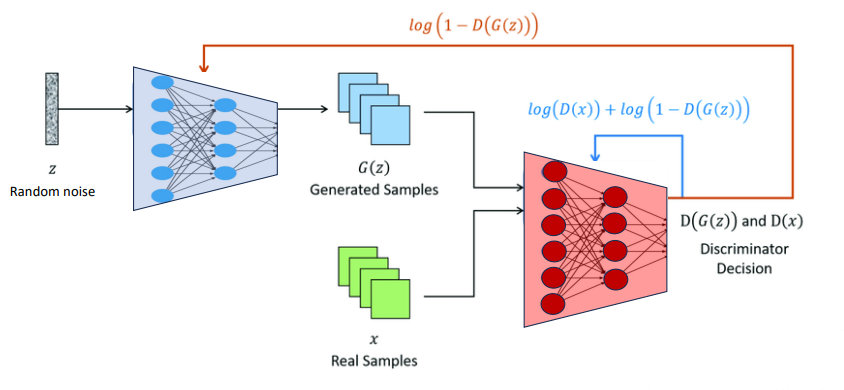
\includegraphics[width=0.5\textwidth]{img/GAN.png}
    \caption{Generative Adversarial Network}
    \label{fig:gan}
\end{figure}

The target of the generator is to generate example the most similar to real one
in such a way to be classified in real example by the discriminator. Quite the
opposite the discriminator have to identify real examples from fake one. If the
discriminator makes a mistake so we will update discriminator's weights, vice
versa we will update generator's weights.
\section{Optimization for training deep models}
When we are creating a deep learning model, we have to consider different aspects
to optimize the training process. In this section, we are going to see some
issues that can arise during the training process and how to solve them.

Let's start by introducing the difference between \textbf{optimization} and
\textbf{machine learning}. In the first case, we are trying to minimize a function
acting directly on it, while in the second case we are trying to minimize a loss
function that is a proxy for the true function we want to minimize.

In machine learning, we aim to optimize a performance measure $P$, based on the
test set. This is done by optimizing a different function $J(\theta)$, with the
hope that improvements in $J(\theta)$ lead to improvements in $P$.

Typically, the loss function is a simple average over the training set and can be
written as:
\begin{equation}
    J(\theta) = E_{(x, y) \approx \hat{P}_{data}} \mathcal{L}(f(x, \theta), y)
\end{equation}
where $\mathcal{L}$ is the loss function, $f$ is the model, $x$ is the input, $y$
is the target and $\theta$ are the parameters of the model. Also, $\hat{P}_{data}$ is
the empirical distribution of the data.

If we know the true data distribution $P_{data}$, the loss function, also called
the \textbf{risk function}, can be expressed as:
\begin{equation}
    J(\theta) = E_{(x, y) \approx P_{data}} \mathcal{L}(f(x, \theta), y)
\end{equation}
and this reduce the machine learning problem to an optimization problem.

The problem of using the empirical distribution is that the model is prone to
overfitting, because we don't have enough data to represent the real distribution.

Instead of minimizing the empirical risk, we can minimize a \textbf{surrogate
    loss function}. This function is a proxy for the true loss function and it
is easier to optimize.

Another difference is that training algorithms doesn't halt at local minima, but
when the early stopping criterion is met. This can be roughly thought of as a
way to reincorporate the true loss function in the learning process.
\subsection{Batch and Minibatch}
One aspect of machine learning algorithms that separates them from general
optimization algorithms is that the objective function usually decomposes as a
sum over the training examples. Computing this expectation exactly is very
expensive, since it requires evaluating the model on every example in the entire
dataset.

However, we can compute these expectations by randomly sampling a small number
of examples from the dataset at every iteration. This works because we are
computing an expected value and, the \textbf{standard error} of the mean estimated
from a sample of size $m$ is:
\begin{equation}
    SE(\mu) = \sqrt{VAR\left[\frac{1}{m}\sum x^{(i)}\right]} = \frac{\sigma}{\sqrt{m}}
\end{equation}
where $\sigma$ is the standard deviation of the distribution. This equation shows
that the relationship is sub-linear between the number of examples and the standard error.

Another consideration that motivates the estimation of the gradient from a
small number of samples is the redundancy in the training set.

Optimization algorithms that use the entire training set to compute the gradient
are called \textbf{batch} or \textbf{deterministic gradient methods}. While the
ones that use a single training example for that task are called \textbf{stochastic
    gradient methods}. Most of the algorithms we use for deep learning fall
somewhere in between and they are called \textbf{mini-batch} or \textbf{mini-batch
    stochastic methods}. We can see the difference between these methods in the
following figure \ref{fig:batchminibatch}.

\begin{figure}[!ht]
    \centering
    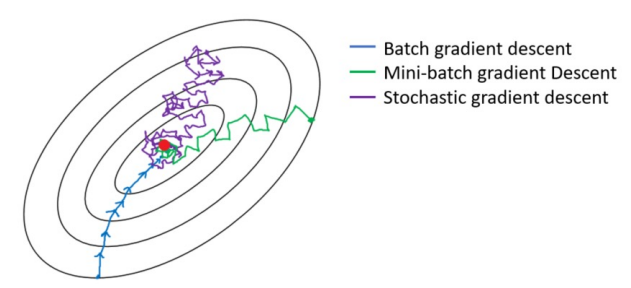
\includegraphics[width=0.5\textwidth]{img/minibatchvsbatch.png}
    \caption{Difference between batch, mini-batch and stochastic gradient methods.}
    \label{fig:batchminibatch}
\end{figure}

In order to chose the right size of the mini-batch, we have to consider that a
larger size will provide a more accurate estimate of the gradient, but with less
than linear improvement in the standard error. While a smaller size will provide
a less accurate estimate of the gradient, but with more than linear improvement
in the standard error and doesn't use the full computational power of the GPU.

\begin{note}
    Usually, a good choice is a power of 2.
\end{note}

It is extremely crucial that mini-batches are sampled at \textbf{random}, because
computing an unbiased estimate of the expected gradient from a set of samples
requires that those samples be independent.

When the order of elements in the dataset holds some significance, it is absolute
necessity to shuffle the examples before selecting every mini-batch.
\subsection{Challenges in deep learning}
Traditionally, machine learning has avoided this difficulty by carefully designing
the objective function and constraints to insure the problem is convex. However,
for training deep models we usually face non-convex optimization.
\subsubsection{Ill-conditioning}
The first challenge is \textbf{ill-conditioning}. This is a problem that arises
when the optimization problem is poorly conditioned. This means that the curvature
of the loss function is very different in different directions.

This condition manifests in stochastic gradient descent when small steps increase
the loss function.

This problem can be identify by looking at the \textbf{condition number} of the
Hessian matrix. If the condition number is very large, we have an ill-conditioned
problem.
\begin{figure}[!ht]
    \centering
    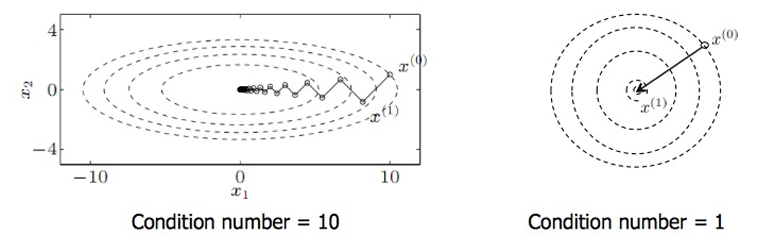
\includegraphics[width=0.5\textwidth]{img/illConditioned.png}
    \caption{Ill-conditioning}
    \label{fig:illconditioning}
\end{figure}

\subsubsection{Local minima}
Functions involved in deep models are guaranteed to have an extremely large
number of local minima. However, we will see that local minima are not
necessarily a major problem because plateaus are an acceptable solution.

Neural networks aren't \textbf{identifiable} there is no single set of parameters
from a single training set. In fact, if we have $m$ layers with $n$ neurons each,
there are $n!^m$ ways to arranging the hidden units to obtain equivalent solutions.
This is called \textbf{weight space symmetry}.

Model identifiability issues mean that there can be an extremely large or even
uncountably infinite amount of local minima in the cost function of deep models.
However, these local minima are all equivalent in value and are not a problematic
form of non-convexity.

Local minima are only truly problematic if they have a much higher cost than the
global minimum.
\subsubsection{Saddle points}
For many high-dimensional non-convex functions, local minima and maxima are in
fact rare compared to \textbf{saddle points}.

A saddle point is a point where the Hessian matrix has both positive and negative
eigenvalues and the gradient is zero. We can think of a saddle point as being a
local minimum along one cross-section of the cost function and a local maximum
along another.

\begin{figure}[!ht]
    \centering
    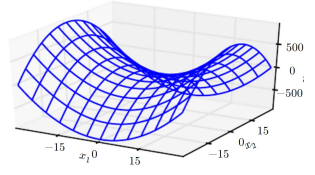
\includegraphics[width=0.5\textwidth]{img/saddle.png}
    \caption{Saddle point}
    \label{fig:saddle}
\end{figure}

This points are more common in high-dimensional spaces than local minima and they
are a problem for optimization algorithms because they are points where the gradient
is zero but they are not a minimum.

For first-order optimization algorithms that use only gradient information, the
situation is unclear. The gradient can often become very small near a saddle point.
On the other hand, gradient descent empirically seems to be able to escape saddle
points in many cases. While, for Newton's Method, saddle points constitute a
major problem, because it actively seeks solutions at critical points where the
gradient is zero.
\subsubsection{Plateaus}
Another problem that can arise during the training process is the presence of
\textbf{plateaus} or \textbf{flat regions}. These are regions where the gradient
is very small and the optimization algorithm can't make progress.
\subsubsection{Cliffs and exploding gradients}
Neural networks with many layers often have extremely steep regions reassembling
cliffs. This regions are the result from the multiplication of many large weights
together.

An extremely steep cliff structure, the gradient update step can move the
parameters extremely far, usually jumping off of the cliff structure altogether.

A solution to this is to use the \textbf{gradient clipping heuristic} which
intervenes to reduce the step size to be small enough that it is less likely to
go outside the region where the gradient indicates the direction of approximately
steepest descent.
\subsubsection{Additional Problems}
There are other problems that can arise during the training process, such as:
\begin{itemize}
    \item \textbf{Long Term Dependencies}: arises when the computational graph
          is very deep. The result of this problem is vanishing and exploding
          gradients.
    \item \textbf{Inexact Gradients}: we usually only have a noisy or even biased
          estimate of the gradient and the Hessian. Sometimes, gradients for our
          loss functions are even intractable. Not a big issue in neural network
          training. Surrogate loss functions tend to perform well enough in practice.
    \item \textbf{Poor Correspondence between Local and Global Structure}: it is
          possible to overcome all of the above problems at a single point and
          still perform poorly if the direction that results in the most
          improvement locally does not point toward distant regions of much
          lower cost.
\end{itemize}
\begin{note}
    The initialization is very important.
\end{note}
\subsection{Optimization algorithms}
There are many optimization algorithms that can be used to train deep models.
In this section, we are going to see some of them.
\subsubsection{Stochastic Gradient Descent}
\textbf{Stochastic Gradient Descent} (SGD) is the most used optimization algorithm
in deep learning. It is based on the idea of computing the gradient of the loss
function on a mini-batch and then update the weights of the model. We can describe
the algorithm as follows:
\begin{itemize}
    \item Sample a mini-batch of examples from the training set.
    \item Compute the gradient of the loss function on the minibatch.
          \begin{equation}
              g \gets \frac{1}{m} \nabla_\theta \sum_{i=1}^m \mathcal{L}(f(x^{(i)}; \theta), y^{(i)})
          \end{equation}
    \item Update the weights of the model using the gradient.
          \begin{equation}
              \theta \gets \theta - \epsilon_k g
          \end{equation}
\end{itemize}
It is important to note that the learning rate $\epsilon_k$ is a hyperparameter
that must be adaptive. This is because the learning rate is a very important
hyperparameter and it can affect the convergence of the algorithm. A sufficient
condition for convergence is:
\begin{equation*}
    \sum_{k=1}^\infty \epsilon_k = \infty \quad \text{and} \quad \sum_{k=1}^\infty \epsilon_k^2 < \infty
\end{equation*}

A common way to implement an adaptive learning rate is to use a linear decay
until the iteration $\tau$. This can be done as follows:
\begin{equation}
    \epsilon_k = \left(1 - \alpha\right)\epsilon_0 + \alpha \epsilon_\tau
\end{equation}
In this case we have to choose three hyperparameter: $\epsilon_0$, $\epsilon_\tau$
and $\alpha$. Usually, $\epsilon_\tau$ is chosen to be $1\%$ of $\epsilon_0$.

To choose $\epsilon_0$ we can try to make different run for a fixed number of
iterations and choose the best one.
\subsubsection{Momentum}
\textbf{Momentum} is a method that helps accelerate SGD in the relevant direction
and dampens oscillations. It is a method that accumulates an exponentially decaying
average of past gradients and continues to move in their direction.

The update rule for momentum is:
\begin{equation}
    \theta \gets \theta + v
\end{equation}
where $v$ is the velocity vector and it is defined as:
\begin{equation}
    v \gets \alpha v - \epsilon \frac{1}{m} \nabla_\theta \sum_{i=1}^m \mathcal{L}(f(x^{(i)}; \theta), y^{(i)})
\end{equation}
where $\alpha$ is the momentum parameter and it is usually set to $0.9$.

This algorithm aims to solve the problem of poor conditioning of the Hessian
matrix, and the variance of stochastic gradients.

The momentum algorithm can be seen as a ball rolling down a hill. The ball
gathers momentum as it rolls down the hill, and it continues to move in the
direction of the momentum even if it encounters a small hill.
\subsubsection{Delta Bar Delta}
\textbf{Delta Bar Delta} is a method that adapts the learning rate for each
parameter. It is based on the following idea:
\begin{itemize}
    \item if the partial derivative of the loss function with respect to a
          parameter remains the same, increase the learning rate.
    \item otherwise, if that partial derivative changes sign, decrease
          the learning rate.
\end{itemize}
\subsubsection{AdaGrad}
\textbf{AdaGrad} is a method that adapts the learning rate for each parameter.
This method scale the gradient according to the historical norms. In this way,
learning of parameters with high partial derivatives decrease faster.

This method is based on the following idea:
\begin{itemize}
    \item Accumulate the square of the gradient into a vector $r$.
          \begin{equation}
              r \gets r + g \odot g
          \end{equation}
    \item Update the weights element wise.
          \begin{equation}
              \Delta\theta \gets - \frac{\epsilon}{\sqrt{r + \epsilon}} \odot g
          \end{equation}
    \item Update parameters
          \begin{equation}
              \theta \gets \theta + \Delta \theta
          \end{equation}
\end{itemize}
\subsubsection{RMSProp}
\textbf{RMSProp} is a method that adapts the learning rate for each parameter.
This method is a modification of AdaGrad to perform better on non-convex problems.
The main difference is that RMSProp use an exponentially weighted moving average.
This method is based on the following idea:
\begin{itemize}
    \item Accumulate the square of the gradient into a vector $r$.
          \begin{equation}
              r \gets \rho r + (1 - \rho) g \odot g
          \end{equation}
    \item Update the weights element wise.
          \begin{equation}
              \Delta \theta \gets - \frac{\epsilon}{\delta + \sqrt{r}} \odot g
          \end{equation}
    \item Update parameters
          \begin{equation}
              \theta \gets \theta + \Delta \theta
          \end{equation}
\end{itemize}
\subsubsection{Adam}
\textbf{Adam} is a variation of RMSProp in which we add the momentum. Also, it
add a bias correction to the moments to account for their initialization at the
origin. This method is based on the following idea:
\begin{itemize}
    \item Update time step:
          \begin{equation}
              t \gets t + 1
          \end{equation}
    \item Update biased moment estimates
          \begin{equation}
              \begin{split}
                  s \gets & \rho_1 S + (1 - \rho_1)g          \\
                  r \gets & \rho_2 r + (1 - \rho_2) g \odot g
              \end{split}
          \end{equation}
    \item Correct biases
          \begin{equation}
              \begin{split}
                  \hat{s} \gets & \frac{S}{1 - \rho_1^t} \\
                  \hat{r} \gets & \frac{r}{1 - \rho_2^t}
              \end{split}
          \end{equation}
    \item Update parameters
          \begin{equation}
              \Delta \theta \gets - \epsilon \frac{\hat{s}}{\delta + \sqrt{\hat{r}}}
          \end{equation}
    \item Update model params:
          \begin{equation}
              \theta \gets \theta + \Delta \theta
          \end{equation}
\end{itemize}
\chapter{Autoencoder}
The \textbf{autoencoder} are neural networks trained to attempt to copy its
input to its output. This is done by a network structured in two parts:
\begin{itemize}
    \item An \textbf{encoder} that maps the input into a hidden-space
    \item A \textbf{decoder} that maps the hidden-space into the output
\end{itemize}

We can represent the autoencoder as a function $h = f(x)$, where $h$ is the
hidden-space representation of the input $x$. The output of the autoencoder is
$g(h)$, where $g$ is the decoder function. The autoencoder is trained to minimize
the difference between the input and the output, i.e. $x \approx g(f(x))$.

This structure is force to select which aspects to preserve and thus hopefully
can learn useful properties of the data.
\section{Types of Autoencoder}
\subsection{Undercomplete Autoencoder}
The simplest form of autoencoder is the \textbf{undercomplete autoencoder}, where
the hidden layer is smaller than the input layer. This forces the autoencoder to
learn a compressed representation of the data.

This model is trained to minimize the reconstruction error, i.e. the difference
between the input and the output. The loss function is usually the mean squared
error (MSE) between the input and the output.
\begin{equation*}
    L(x, g(f(x))) = ||x - g(f(x))||^2
\end{equation*}
\begin{note}
    If we have a linear activation function, the undercomplete autoencoder is
    equivalent to the PCA.
\end{note}

We could have non linear autoencoder, where the encoder and decoder are non-linear
functions. This allows the autoencoder to learn more complex representations of
the data.
\subsection{Regularized Autoencoder}
\textbf{Regularized autoencoder} are autoencoder that are trained to minimize the
reconstruction error, but also have a regularization term. This term is used to
prevent the autoencoder from learning the identity function.

This can be subdivided into:
\begin{itemize}
    \item \textbf{Sparse autoencoder}: is a regularized autoencoder where the
          hidden layer is greater than the input layer. Usually we add a
          regularization term to the loss function to penalize the activation
          of the hidden units.This type must respond to statistical features of
          the dataset, ratehr than acting as an identity function.
    \item \textbf{Denoising autoencoder}: are basic autoencoder where the task
          is to reconstruct the input without noise. The input is corrupted by
          adding some noise, and the autoencoder is trained to reconstruct the
          original input.
    \item \textbf{Stacked autoencoder}: are autoencoder where the encoder and
          decoder are composed of multiple layers. This allows the autoencoder
          to learn more complex representations of the data.
    \item \textbf{Variational Autoencoder}: are autoencoder that are trained to
          learn the parameters of the probability distribution that generates
          the data. This allows the autoencoder to generate new data similar to
          the training data. The middle layer of the autoencoder is used to
          represent the mean and the variance of the distribution. And, the loss
          function need to be improved to take into account the difference between
          the probability distribution of the input and the output.
\end{itemize}
\chapter{Convolutional Neural Network}
\textbf{Convolutional Neural Network} (CNN) are particular types of neural network
feed forward. Their goal is to use multiple layers, stacked one on top of the other,
in order to extract input-related features. These layers are organized in a
hierarchical way, where the highest level calculates more global, more invariant
features.

Unlike the networks seen so far, CNNs organize weights using 3 dimensions. From
this point on, we will talk about the weights also considering the \textbf{volume}.
These volumes arise because the input consists of spatial dimensions (image width and
height) along with multiple input channels (e.g., RGB for color images). Each
neuron in a CNN acts as a filter, processing the entire spatial dimensions and
all input channels simultaneously. The output of each layer is another volume,
where the depth corresponds to the number of filters (or neurons) in the hidden
layer.

\begin{figure}[!ht]
    \centering
    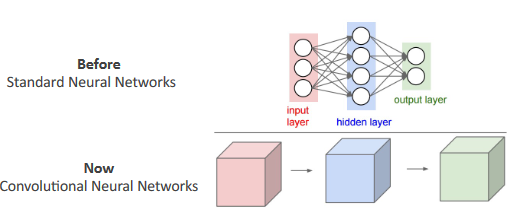
\includegraphics[width=0.5\textwidth]{img/CNN/weights.png}
    \caption{Weights representation in Feed Forward vs CNN.}
    \label{fig:weights}
\end{figure}

This particular type of network is widely used in the field of digital signal
processing, such as image or audio signals. If we look at image processing, this
kind of neural network offers a much more cost-effective approach than traditional
feed forward.

The most significant difference lies in how connections are structured. In a
feed forward network, each input neuron is fully connected to all neurons in the
next layer. This results in a significant complexity challenge. For instance,
with an image of $100 \times 100$ pixels, the input to the network is a vector
of $10,000$ pixels, leading to an enormous number of connections.

CNNs, on the other hand, introduce local connectivity, where each neuron focuses
on a small, localized portion of the image in each channel (\textbf{Local
    connectivity}). This drastically reduces the number of neurons and connections
required. For example, if the input image has dimensions $1000 \times 1000 \times 3$
(width, height, and 3 color channels), a single neuron could use a $5 \times 5 \times 3$
set of parameters. This is because the neuron processes a $5 \times 5$ spatial
region across all channels of the previous layer, a property referred to as full
depth connectivity.

\begin{figure}[!ht]
    \centering
    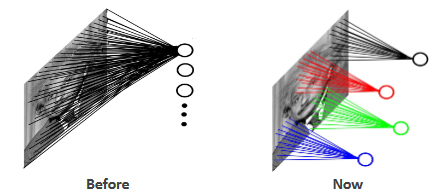
\includegraphics[width=0.5\linewidth]{img/CNN/localConn.png}
    \caption{Difference between the connections of neurons in a feed forward
        network and a CNN.}
    \label{fig:localConn}
\end{figure}

Also, another difference is that now, we have neurons organized in depth, we have
multiple neurons all looking the same region of the input volume, stacked along depth.

\begin{figure}[!ht]
    \centering
    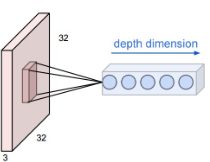
\includegraphics[width=0.25\linewidth]{img/CNN/depth.png}
    \caption{Organization of neurons in CNN}
    \label{fig:depth}
\end{figure}

In total we have $5\times 5\times 3$ weights to learn shared between each patch
of the image, this reduce a lot the number of learning parameter compared to
feed forward network. This concept is called \textbf{weights sharing}, which means
that the weights in the layer are shared across spatial positions.

In general, the structure of a CNN is organized so that it has a first part,
which includes convolutional layers, that extract the main characteristics from
the input. There is then a second part, composed of fully connected layer, which
performs the actual classification task. We can then represent this type of
network with a structure like the one shown in figure \ref{fig:cnnarc}.

\begin{figure}[!ht]
    \centering
    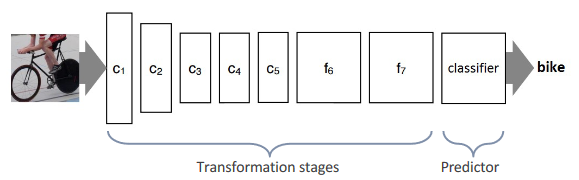
\includegraphics[width=\linewidth]{img/CNN/CNNarc.png}
    \caption{Overall CNN architecture.}
    \label{fig:cnnarc}
\end{figure}

The concept of \textbf{backpropagation} can still be utilized with this
architecture, which is a crucial aspect of training CNNs.

Respect to traditional neural networks, CNNs incorporate additional specialized
layers, such as \textbf{Spatial pooling} and \textbf{Local response normalization}.

These layers are useful to reduce computational complexity, increase invariance
and ease the optimization.
\section{CNNs components}
\subsection{Linear Convolution}
We begin by introducing the concept behind convolutional networks, namely the
concept of \textbf{linear convolution}. Convolution is a linear, local
(it applies on patches) and translation-invariant operator. To enrich the data
representation, we can use a \textbf{filter bank}, that is a collection of $Q$
sets of $K$ filters that allows to produce an output of $Q$ channel.

Let's see now, on a more mathematical level, what convolution represents. First we
introduce what we need:
\begin{itemize}
    \item $x = H \times W \times K$ is our input where $H$ represents the height
          dimension, $W$ the width dimension and $K$ the number of channels.
    \item $F = H' \times W' \times K \times Q$ is our filter bank where $Q$ is
          the number of filters that need to be apply to each channel.
    \item $y = (H - H' + 1) \times (W - W' + 1) \times Q$ is our output.
\end{itemize}

In addition to these, another very important thing to define is the \textbf{stride}.
The stride determines the step size for moving the filter across the input. By
default, the stride is set to 1, meaning the filter's center moves one pixel at
a time before being applied again.

\begin{note}
    A filter bank with 16 filters of depth $K$ produces an output with 16 channels.
\end{note}

The convolution is expressed by the following formula:
\begin{equation}
    y_{i, j, q} = y_q + \sum_{u = 0}^{H - 1}\sum_{v = 0}^{W - 1}\sum_{k = 1}^{K} x_{u + i, v + j, k} \cdot F_{u, v, k, q}
\end{equation}
where:
\begin{itemize}
    \item $y_q$ is the bias of the filter $F_q$;
    \item $x_{u + i, v + j, k}$ is the input patch of channel $k$;
    \item $F_{u, v, k, q}$ is the filter for the channel $k$ that computes output
          channel $q$.
\end{itemize}

\begin{figure}[!ht]
    \centering
    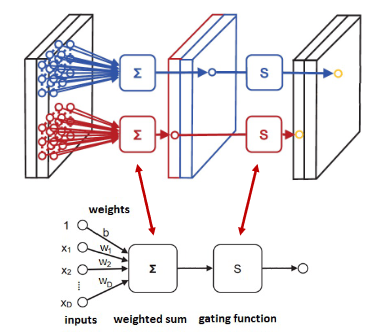
\includegraphics[width=0.25\linewidth]{img/CNN/Conv2Filter.png}
    \caption{Example of convolutional network with a filter bank of two elements.}
    \label{fig:conv2filter}
\end{figure}

We can apply filters in 2 way:
\begin{itemize}
    \item \textbf{Lattice structure}: a single filter is applied to a single
          channel ($K = 1$);
    \item \textbf{Multiple feature structure}: a single filter is applied to all
          channel of the input image $(K > 1)$.
\end{itemize}

In CNN, after the filter application we use a non linear activation function,
also called \textbf{gating function}: \textit{Sigmoid}, \textit{Tanh}, \textit{ReLU}
and \textit{SmoothReLU}.

\subsection{Spatial pooling}
We have already said that there are different types of layers in a CNN, one of
them is the \textbf{spatial pooling}.

The purpose of this layer is to subsample the image, reducing its spatial
dimensions and, in turn, the computational load. Additionally, spatial pooling
aggregates information from the image, enhancing translation invariance, which
makes the model more robust to variations in the exact spatial positions of
features. This is done in two main ways:
\begin{itemize}
    \item \textbf{avg pooling}: computing an average of the value of the pixels
          in the neighborhood:
          \begin{equation}
              y_{ijk} =\text{avg}_{p, q \in \Omega} x_{p, q, k}
          \end{equation}
    \item \textbf{max pooling}: taking the maximum value from the pixels in the
          neighborhood:
          \begin{equation}
              y_{ijk} = \max_{p, q \in \Omega_{i, j}} x_{p, q, k}
          \end{equation}
\end{itemize}

This is done channel by channel.
\subsection{Local Response Normalization}
\textbf{Local Response Normalization} layers have the objective of normalizing the
effect of contrast to improve the network invariance in this respect. This layer
also allows for improved optimization and sparsity (accuracy and speed).

In general, there are two ways of applying it:
\begin{itemize}
    \item \textbf{Within Channel}: operates independently on different feature
          channels, and also rescales each input feature basing on a local
          neighborhood.
          \begin{equation}
              y_{i, j, k} = x_{i, j, k} \left(k + \alpha \sum_{(u, v) \in \mathcal{N}(i, j)} x_{u, v, k}^2 \right)^{-\beta}
          \end{equation}
    \item \textbf{Across Channels}: operates independently at each spatial location
          and groups of channels. It also normalizes groups $G(k)$ of feature
          channels. Groups are usually defined in a sliding window manner.
          \begin{equation}
              y_{i, j, k} = x_{i, j, k} \left(k + \alpha \sum_{q \in G(k)} x_{i, j, q}^2 \right)^{-\beta}
          \end{equation}
\end{itemize}

\subsection{Input sensibility}
CNN are sensible to the input images, moreover we need a lot of data to train
from scratch a CNN. So we have to normalize images using:
\begin{itemize}
    \item \textbf{Local mean subtraction}
    \item \textbf{Normalization}
\end{itemize}
to have data centered in 0. To prevent overfitting we can use:
\begin{itemize}
    \item Weight decay;
    \item Dropout;
    \item Data augmentation: for example changing illuminants, flip the image,
          random crop and a geometric distortion.
\end{itemize}
Remember that is always better to accept new data.

\section{CNN Architectures}
Below, we will introduce some of the most famous CNN architectures. This is done
because the training from zero of one of these models requires a very large amount
of data and many computational resources.
\begin{itemize}
    \item \textbf{LeNet} is one of the first model that this is first create for
          the MNIST dataset. This network take in input a gray scale image of
          size $32 \times 32$.
          \begin{figure}[!ht]
              \centering
              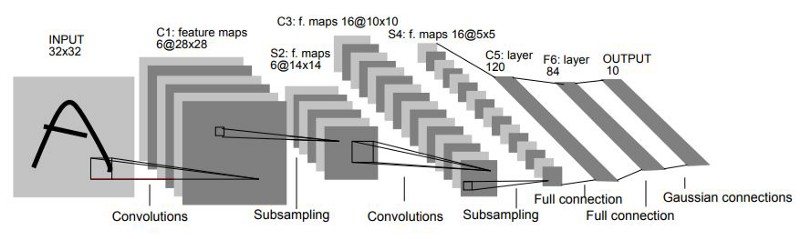
\includegraphics[width=0.45\linewidth]{img/CNN/LeNet-5.jpeg}
              \caption{LeNet}
              \label{fig:lenet}
          \end{figure}
    \item \textbf{AlexNet} was created for the ImageNet challenge and combines
          some convolutional layers with feed forward layers. It starts with a
          large convolutional level that is gradually reduced in order to encode
          the deeper layers of the more specific information in the task. In
          general we decrease filter dimension, increasing the depth channels.
          \begin{figure}[!ht]
              \centering
              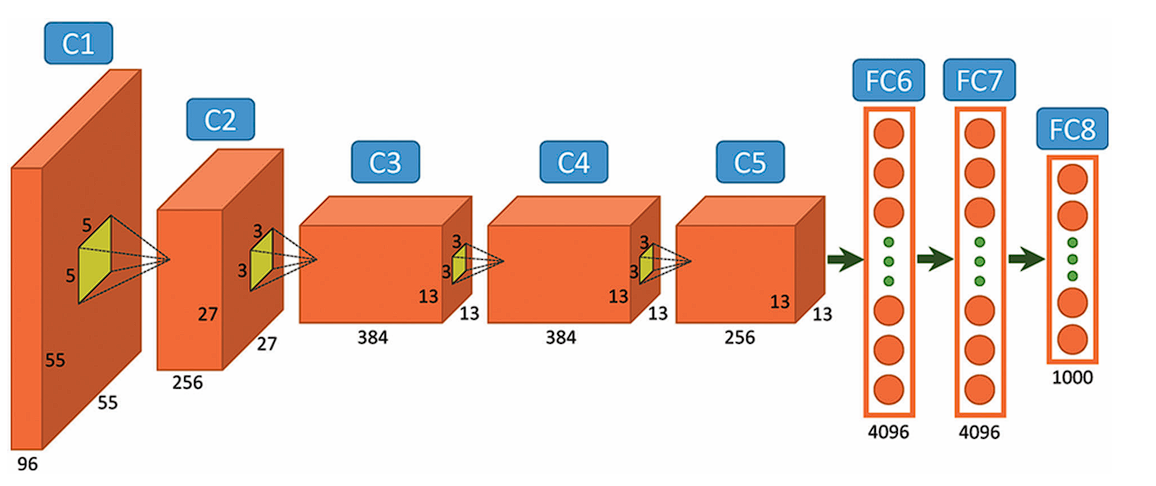
\includegraphics[width=0.45\linewidth]{img/CNN/alexNet.png}
              \caption{AlexNet}
              \label{fig:alexnet}
          \end{figure}
    \item \textbf{VGG} is a family of CNNs that consists of networks with varying
          numbers of convolutional layers. Compared to AlexNet, VGG uses smaller
          filters to reduce the number of parameters. Additionally, due to the
          concept of the \textbf{receptive field}, using smaller filters in multiple
          layers can achieve a similar receptive field to using a larger filter
          in a single layer. This allows VGG to maintain model depth while managing
          the number of parameters more efficiently.
          \begin{figure}[!ht]
              \centering
              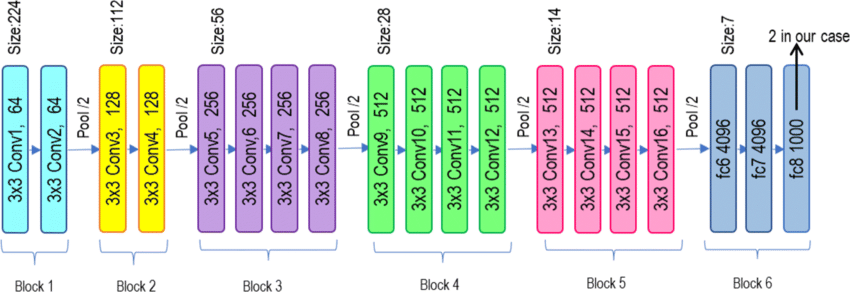
\includegraphics[width=0.45\linewidth]{img/CNN/VGG.png}
              \caption{VGG-19}
              \label{fig:vgg}
          \end{figure}
    \item \textbf{GoogLeNet} is one of the first networks to introduce the
          \textbf{module} concept. In particular, it uses the module called
          \textbf{inception} which is a part of the network, which can be stacked
          over other similar modules to get a larger network.

          As we are increasing the size of the network, we may encounter the
          problem of vanishing gradient. To solve this problem the creators introduce
          auxiliary output levels in different parts of the network in order to
          inject the gradient into different levels.

          This is done by creating a loss function which is a linear combination
          of the output, with an higher weights on final loss than the others losses.
          \begin{figure}[!ht]
              \centering
              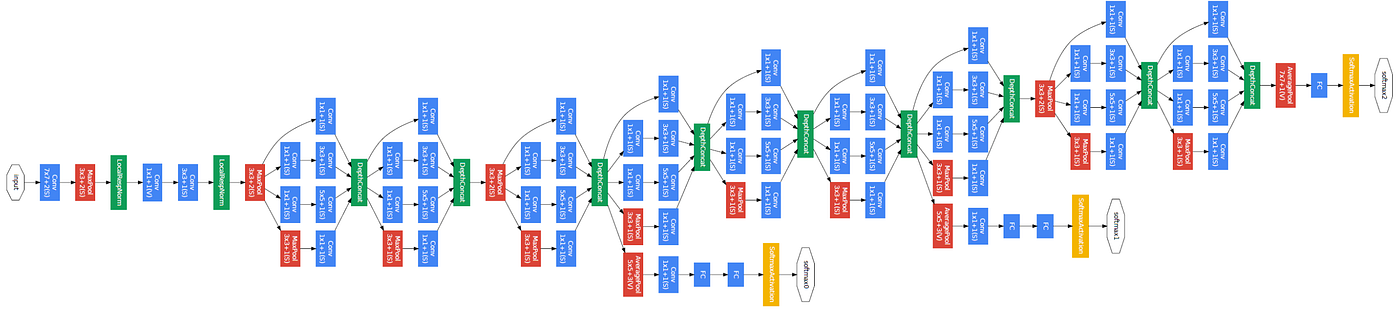
\includegraphics[width=0.45\linewidth]{img/CNN/GoogLeNet.png}
              \caption{GoogLeNet}
              \label{fig:GoogLeNet}
          \end{figure}
    \item \textbf{ResNet} is a network type that uses the idea of \textbf{residue}.
          The basic concept is to provide in input the identity function and let
          the network learn how to modify this function to approach the one you
          want to learn. The identity function is used because it can be easily
          implemented by adding the input to the result obtained at a particular
          point in the network. This is done to limit the vanishing gradient
          problem as the derivative of the identical function is always 1. With
          this trick you can implement much deeper networks.
          \begin{figure}[!ht]
              \centering
              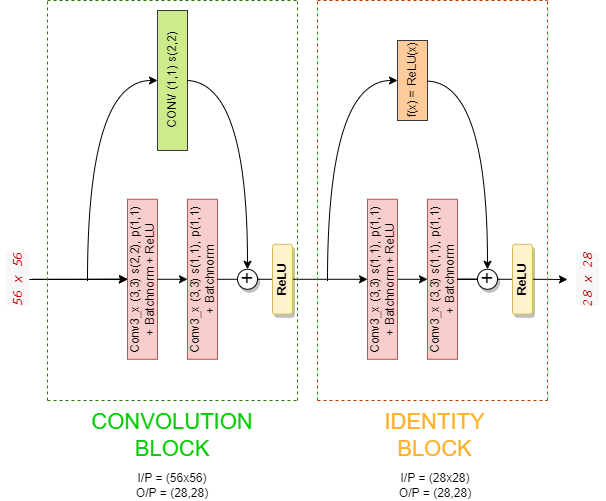
\includegraphics[width=0.25\linewidth]{img/CNN/ResNet.png}
              \caption{ResNet}
              \label{fig:resnet}
          \end{figure}
\end{itemize}

\begin{note}
    Usually we can use $1 \times 1$ convolution to squeeze information in depth
    channel without having impact on the spatial information.
\end{note}

\subsection{Transfert learning}
As mentioned above, it is not always possible to train a CNN from scratch. Depending on
the situation and the amount of data available. Generally we can train model from
scratch on a big dataset, then we can fine tune on our task dataset. In general,
one of the following techniques may be adopted:
\begin{itemize}
    \item New dataset is small and similar to original dataset: we can train a
          linear classifier on CNN features from higher layers;
    \item New dataset is large and similar to original dataset: we can Fine-tune
          the CNN;
    \item New dataset is small but very different from original dataset: we can
          train a linear classifier on CNN features from lower layers because we
          have to learn general features;
    \item New dataset is large and very different from original dataset: we can
          train CNN from scratch or fine-tune it
\end{itemize}

\section{Model Compression}
When developing a Deep Neural Network model, it is crucial to consider the devices
on which it will run, especially if the model is to be distributed to users. For
example, running a large language model (LLM) on a mobile device would not be
practical. Therefore, it's important to find the right balance between performance
and compatibility. One possible solution is to host the model in the cloud, but
this approach introduces challenges, such as network latency and privacy concerns.

An alternative approach is to create a more compact model that can run efficiently
on a mobile device while achieving performance similar to that of larger models.
An added advantage of this solution is that, due to its reduced size, the inference
process will be faster.

To achieve these results, several aspects were studied.
\subsection{Weight Sharing}
\textbf{Weight sharing} is a simple form of network reduction that involves
sharing weights between layers or structures within layers. Unlike other
compression techniques, weight sharing is typically applied before training the
original network, rather than compressing the model after training. This technique
reduces the network size and avoids sparsity. However, it is not always clear
how many and which weights should be shared before performance degradation becomes
unacceptable for a given network architecture and task.

An example of weight sharing can be seen in Convolutional layers, where each
neuron shares the same set of weights.

\subsection{Network pruning}
Pruning weights is one of the most commonly used techniques to reduce the number
of parameters in a pre-trained Deep Neural Network (DNN). This can lead to
reductions in storage and model runtime. Performance is usually maintained by
retraining the pruned network.

Iterative weight pruning prunes weights while retraining the network until the
desired trade-off between network size and accuracy is achieved. The simplest
pruning strategy involves setting a threshold to determine which weights or units
(in this case, the absolute sum of the magnitudes of incoming weights) are
removed. The threshold can vary for each layer or be global for the entire network.
Instead of setting a threshold, one can predefine a percentage of weights to be
pruned based on their magnitude, or a percentage aggregated by weights for each
layer. Typically, the weights with magnitudes closest to 0 are removed.

\textbf{Magnitude-based pruning (MBP)} is the most commonly used pruning technique
in DNNs due to its simplicity. It works well for a wide range of machine learning
models, including DNNs, across various tasks. In general, global MBP tends to
outperform layer-wise MBP because it provides more flexibility in determining
the amount of sparsity for each layer. This allows more important layers to remain
denser while less important layers contain more non-zero entries.

\subsubsection{Categorization of Pruning Techniques}
\begin{itemize}
    \item \textbf{Magnitude-based (iterative pruning + retraining)}: This technique
          removes the weights with the lowest absolute values based on a set
          threshold or percentage, either layer-wise or globally. The steps are
          as follows:
          \begin{enumerate}
              \item Choose a neural network architecture.
              \item Train the network until a reasonable solution is obtained.
              \item Prune the weights with magnitudes smaller than a threshold $\tau$.
              \item Retrain the network until a reasonable solution is obtained.
              \item Repeat step 3.
          \end{enumerate}
    \item \textbf{Methods that penalize the objective} with a regularization
          (L1, L2, etc.) term to force the model to learn a network with smaller
          weights and prune the smallest weights. This pruning technique is based
          on weight regularization, where we add a penalty term to the objective
          function to encourage the model's weights to approach zero. The smallest
          weights are then deleted. Typically, an L2 regularization is used, but
          care should be taken when using a more quadratic penalty as it can overly
          penalize larger weights.
    \item \textbf{Methods that compute the sensitivity of the loss function} when
          weights are removed, using this sensitivity as a criterion for removing
          weights that result in the smallest change in loss. \textbf{(Diagonal)
              Hessian-based pruning: Optimal Brain Damage}:
          \begin{enumerate}
              \item Choose a neural network architecture.
              \item Train the network until a reasonable solution is obtained.
              \item Compute the second derivatives for each parameter.
              \item Compute the saliencies for each parameter: $S_k = \frac{\delta^2E}{\delta^2 u_k} u_k^2$.
              \item Sort the parameters by saliency and delete low-saliency parameters.
              \item Repeat step 2.
          \end{enumerate}
    \item \textbf{Search-based approaches} that seek to learn or adapt a set of
          weights, links, or paths within the neural network, keeping those that
          are salient for the task.
\end{itemize}
\subsubsection{Structured vs. Unstructured Pruning}
Another important distinction to be made is between structured and unstructured
pruning techniques:
\begin{itemize}
    \item \textbf{Structured pruning} aims to preserve network density for
          computational efficiency (resulting in faster computation at the expense
          of less flexibility) by removing groups of weights.
    \item \textbf{Unstructured pruning} is unconstrained as to which weights or
          activations are removed, but the sparsity means that the dimensionality
          of the layers does not change.
\end{itemize}
Therefore, sparsity in unstructured pruning techniques generally provides good
performance at the expense of slower computation.

\textbf{Structured pruning via weight regularization}: Since standard pruning
leads to non-structured connectivity, structured pruning can be used to reduce
memory usage and increase speed. Hardware is more amenable to dealing with dense
matrix multiplications, especially when there are few non-zero entries in matrices
and tensors. Convolutional Neural Networks (CNNs) are particularly suitable for
this type of pruning since they consist of sparse connections.

\textbf{Group sparsity regularization}: Group sparse regularizers enforce a subset
of weight groupings (such as filters in CNNs) to be close to zero when trained
using stochastic gradient descent. For example, consider a convolutional kernel
represented as a tensor $K(i; j; s; :)$. The group-wise $L_1$-norm, $L_2$-norm
is given as:
\begin{equation*}
    \omega_{2, 1}(K) = \lambda \sum_{i, j, s} | \Gamma_{ijs} | = \lambda \sum_{i, j, s} \sqrt{\sum_{t= 1}^T K(i, j, s, t)^2}
\end{equation*}

Where $\Gamma_{ijs}$ is the group of kernel tensor entries $K(i; j; s; :)$, where
$(i;j)$ represents the pixel location in the $i$-th row and $j$-th column of the
image for the $s$-th input feature map. This regularization term forces certain
groups $\Gamma_{ijs}$ to be close to zero, which can be useful for pruning.

\subsection{Low rank matrix and tensor decomposition}
The idea starts from the observation that most weights are in the fully connected
layers, and that fully connected layers are implemented with a single matrix
multiplication.
\subsection{Knowledge distillation}
Involves learning a smaller network from a large network using supervision from
the larger network and minimizing the entropy, distance or divergence between
their probabilistic estimates. Probably the first work about KD is from Bucilua
et al. where they explored the idea of reducing model size by learning a student
network from an ensemble of models.
\begin{itemize}
    \item They use a teacher network to label a large amount of unlabeled data
          and train a student network using supervision from the pseudo labels
          provided by the teacher;
    \item They find performance is close to the original ensemble with $1000 \times$
          smaller network.
\end{itemize}

Hinton et al. showed a neural network knowledge distillation approach where a
small model is trained using supervision (class probability outputs) from the
original “teacher” model. They showed that learning from the larger network
outperformed the smaller network learning from scratch in the standard supervised
classification setup.
\subsection{Quantization}
\textbf{Quantization} is the process of representing values with a reduced number
of bits. In neural networks, this can be applied to weights, activations and
gradient values. Typically, when training on the GPU, values are stored in 32-bit
floating point (FP) single precision. Half-precision for floating point (FP-16)
and integer arithmetic (INT-16) are also commonly considered. INT-16 provides
higher precision but a lower dynamic range compared to FP-16. In FP-16, the result
of a multiplication is accumulated into a FP-32 followed by a down-conversion to
return to FP-16.

To speed up training, faster inference and reduce bandwidth memory requirements,
ongoing research has focused on training and performing inference with lower-precision
networks using integer precision (IP) as low as INT-8, INT-4, INT-2 or 1 bit
representations.

Designing such networks makes it easier to train such networks on CPUs, FPGAs,
ASICs and GPUs. Two important features of quantization are the range of values
that can be represented and the bit spacing.

For the range of signed integers with n bits, we represent a range of $[-2n-1, 2n-2]$
and for full precision (FP-32) the range is $\pm3.4e38$. For signed integers,
there are $2n$ values in that range and approximately $4.2e9$ for FP-32. FP can
represent a large array of distributions which is useful for neural network
computation, however this comes at larger computational costs when compared
to integer values.

For integers to be used to represent weight matrices and activations, a FP scale
factor is often used hence many quantization approaches involve a hybrid of mostly
integer formats with FP-32 scaling numbers. This approach is often referred to
as mixed-precision (MP). Different MP strategies have been used to avoid overflows
during training and/or inference of low resolution networks given the
limited range of integer formats.
\subsection{Low resource and efficient architectures}
\begin{figure}[!ht]
    \centering
    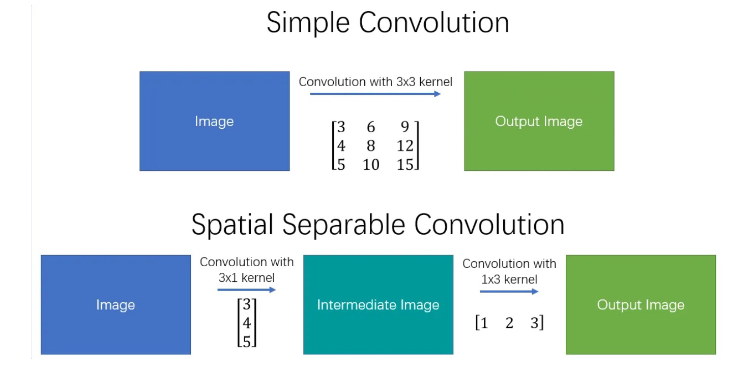
\includegraphics[width=0.5\linewidth]{img/CNN/spatialConv.png}
    \caption{Spatial Separable Convolution}
    \label{fig:spatialConv}
\end{figure}
\begin{itemize}
    \item \textbf{MobileNet}: is a sort of compression of CNN for embedded mobile
          vision application. They use depth-wise separable convolution (DSC) and
          2 hyperparameter that trade off latency and accuracy. DSC split the
          convolution in 2 steps, first filtering then combining outputs of each
          DSC filter, this is why it is referred as factorization approach.
    \item \textbf{SqueezeNet}: reduce the network architecture by reducing $3 \times 3$
          filters to $1\times1$ filters (squeeze layer). Reduce the number of
          input channels to $3 \times 3$ filters using squeeze layers and down
          sample later in the network to avoid the bottleneck of information
          through the network too early and in turn lead to better performance.
          A fire module is made up of the squeeze layer and an expand layer that
          is a mix of $1 \times 1$ and $3 \times 3$ convolution filters. The number
          of filters per fire module is increased as it gets closer to the
          last layer.
    \item \textbf{ShuffleNet}: uses point-wise group convolutions (i.e using a
          different set of convolution filter groups on the same input features,
          this allows for model parallelization) and channel shuffles (randomly
          shuffling helps information flow across feature channels) to reduce
          compute while maintaining accuracy. ShuffleNet is made up economical
          $3 \times 3$ depth-wise convolutional filters and replace $1 \times 1$
          layer with point-wise group convolutional followed by the channel
          shuffle. Unlike predecessor models, ShuffleNet is efficient for smaller
          networks.
    \item \textbf{DenseNet}: Gradients can vanish in very deep networks because
          the error becomes more difficult to backpropagate as the number of
          matrix multiplications increases. DenseNets address gradient vanishing
          connecting the feature maps of the previous layer to the inputs of the
          next layer, similar to ResNet skip connections. This reusing of features
          means the network efficient with its use of parameters. Although, deep
          and thin DenseNetworks can be parameter efficient, they do tradeoff
          with memory/speed efficiency in comparison to shallower yet wider network
          because all layer outputs need to be stored to perform backpropagation.
          However, DenseNets too can be made wider and shallower to become more
          memory efficient if required.
\end{itemize}
\chapter{Recurrent Neural Networks}
\textbf{Recurrent Neural Networks} (RNN) are a family of neural networks for
processing sequential data. It is specialized for processing sequence of values
$x^{(1)}, \dots, x^{(\tau)}$. Recurrent networks can scale to much longer sequences
than would be practical for networks without sequence-based specialization. Most
recurrent networks can also process sequences of variable length.

To go from multilayer networks to recurrent networks, we need to take advantage
of one of the early ideas: sharing parameters across different parts of a model.
Parameter sharing makes it possible to extend and apply the model to examples of
different forms (different lengths, here) and generalize across them.

Recurrent networks share parameters differently compared to CNNs. Each output
member is a function of the previous output members and is produced using the
same update rule applied recursively to the earlier outputs. This recurrent
formulation leads to parameter sharing across a very deep computational graph.

Usually, RNN are defined using computational graph (CG) (Figure \ref{fig:rnn}).
In particular, in the Figure \ref{fig:rnn} we used the following notation:
\begin{itemize}
    \item $x^{(i)}$ is a value of the input sequence;
    \item $h^{(i)}$ represent the hidden layers;
    \item $o^{(i)}$ represent the output layer;
    \item $y^{(i)}$ represent the training target;
    \item $L^{(i)}$ is the loss that measures how far each $o$ is from the
          corresponding training target $y$.
\end{itemize}
The RNN has input-to-hidden connections parametrized by a weight matrix $\textbf{U}$,
hidden-to-hidden recurrent connections parametrized by a weight matrix $\textbf{W}$,
and hidden-to-output connections parametrized by a weight matrix $\textbf{V}$.

RNN uses the information coming from previous hidden layers to compute actual
prevision. There are also variants whose only occurrence is the feedback link
from the output to the hidden layer (Figure \ref{fig:rnn1}). This mechanism
implements \textbf{memory} behaviors.


This architecture is designed to apply the same operations to all the data of the
sequence. All inputs and outputs are dependent, because we apply the same operation
on all data using past operations.

There are different architectures of RNN:
\begin{itemize}
    \item RNNs that produces output for each time step and the recurrent connection
          from the previous hidden layer to the next hidden layer. (Figure \ref{fig:rnn})
    \item RNN that produces output for each time step and the recurrent connection
          is from output to the next hidden layer. (Figure \ref{fig:rnn1})
    \item RNN that doesn't produce output for each time step, but we have the
          recurrent connection from output to the next hidden layer. At the end
          of the sequence we produce output. (Figure \ref{fig:rnn2})
\end{itemize}

\begin{figure}[!ht]
    \centering
    \begin{subfigure}[b]{0.3\textwidth}
        \centering
        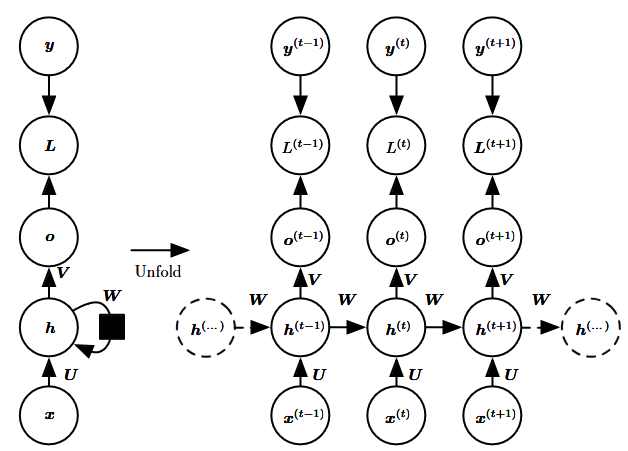
\includegraphics[width=\linewidth]{img/RNN/RNN.png}
        \caption{The computational graph of a recurrent network}
        \label{fig:rnn}
    \end{subfigure}
    \hfill
    \begin{subfigure}[b]{0.3\textwidth}
        \centering
        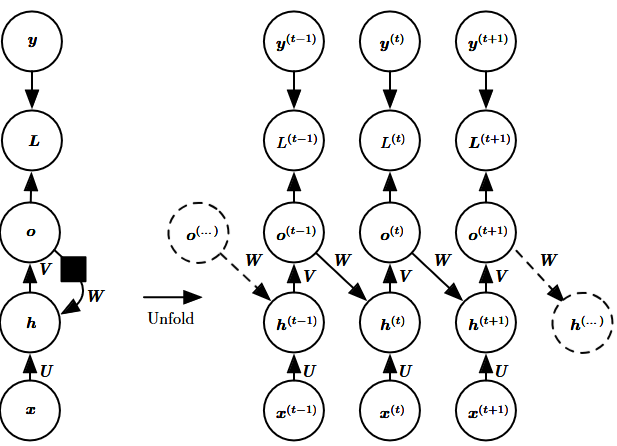
\includegraphics[width=\linewidth]{img/RNN/RNN1.png}
        \caption{An RNN whose only recurrence is the feedback connection from the
            output to the hidden layer.}
        \label{fig:rnn1}
    \end{subfigure}
    \hfill
    \begin{subfigure}[b]{0.3\textwidth}
        \centering
        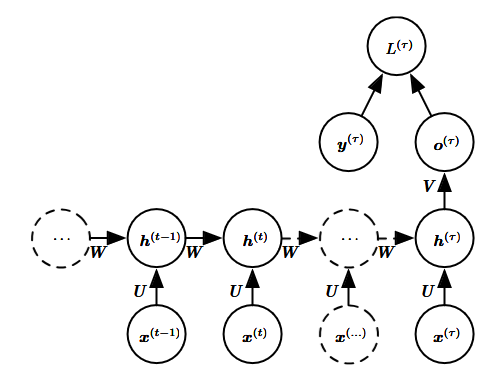
\includegraphics[width=\linewidth]{img/RNN/RNN2.png}
        \caption{Recurrent neural network with a single output at the end of the sequence}
        \label{fig:rnn2}
    \end{subfigure}
\end{figure}

The use of multiple layers in various parts of an RNN—input, hidden, and output
layers—can enhance performance; however, there is currently no theoretical proof
to support this.

To train such models, we can apply a similar approach to the architectures discussed
previously. However, some adjustments are necessary, as the information is derived
not only from the input layers but also from past hidden layers.

Computing the gradient of this loss function with respect to the parameters is an
expensive operation. The gradient computation involves performing a forward
propagation pass moving left to right through our illustration of the unrolled
graph, followed by a backward propagation pass moving right to left through
the graph. The runtime is $\mathcal{O}(\tau)$ and cannot be reduced by parallelization
because the forward propagation graph is inherently sequential; each time step
may be computed only after the previous one. States computed in the forward pass
must be stored until they are reused during the backward pass, so the memory cost
is also $\mathcal{O}(\tau)$. The back-propagation algorithm applied to the unrolled
graph with $\mathcal{O}(\tau)$ cost is called \textbf{back-propagation through time} (BPTT).

For notation purposes let's use $o^{(t)} =  \hat{y}^{(t)}$ Then consider:
\begin{equation}
    h^{(t)} = \tanh (U \cdot x^{(t)} + W \cdot h^{(t - 1)}) \,\, \land \,\, \hat{y}^{(t)} = softmax(V \cdot h^{(t)})
\end{equation}
And the cross entropy as the loss (i.e., error) function to minimize:
\begin{equation}
    E(y, \hat{y}) = \sum_t E^{(t)}(y^{(t)}, \hat{y}^{(t)}) = - \sum_t y^{(t)} \cdot \log(\hat{y}^{(t)})
\end{equation}

The goal of BPTT is to calculate the gradients of the error with reference to
$U, V, W$ and then learn good values of these parameters using Stochastic Gradient
Descent. Just like we sum up the errors, we also sum up the gradients at each
time step for one training example:
\begin{equation}
    \frac{\partial E}{\partial U} = \sum_t \frac{\partial E^{(t)}}{\partial U}, \,\, \land \,\,
    \frac{\partial E}{\partial V} = \sum_t \frac{\partial E^{(t)}}{\partial V}, \,\, \land \,\,
    \frac{\partial E}{\partial W} = \sum_t \frac{\partial E^{(t)}}{\partial W}
\end{equation}

To calculate these gradients, we use the differentiation chain rule, which
underpins the (traditional) backpropagation algorithm. While the computation of
$\frac{\partial E}{\partial V}$ may be relatively straightforward depending on
the RNN architecture, applying the chain rule to compute $\frac{\partial E}{\partial U}$
and $\frac{\partial E}{\partial W}$ is much more complex. This is because we must
backpropagate the gradients from the output, through the network, and all the way
back to $t = 0$.

The basic problem is that gradients propagated over many stages tend to either
\textbf{vanish} (most of the time) or \textbf{explode} (rarely, but with much
damage to the optimization). The difficulty with long-term dependencies arises
from the exponentially smaller weights given to long-term interactions (involving
the multiplication of many matrices) compared to short-term ones.

One might hope to avoid the problem by staying in a region of parameter space where
gradients neither vanish nor explode. Unfortunately, for the RNN to store memories
in a manner robust to small perturbations, it must enter a region of parameter
space where gradients vanish. Specifically, whenever the model can represent
long-term dependencies, the gradient of a long-term interaction has an exponentially
smaller magnitude compared to the gradient of a short-term interaction. This does
not mean it is impossible to learn long-term dependencies, but rather that it
might take a very long time, as the signal associated with these dependencies is
often overshadowed by the smallest fluctuations arising from short-term dependencies.

Since we need to compute a product of gradients at each time step, we may encounter
one of the following issues:
\begin{itemize}
    \item \textbf{Exploding gradients}: This occurs when all gradients are $> 1$.
          It can be mitigated by gradient clipping;
    \item \textbf{Vanishing gradients}: This arises when all gradients are $< 1$,
          leading to challenges in training. Solutions include using appropriate
          activation functions, weight initialization strategies, or modifying
          the network architecture, with the latter being the most effective
          approach for addressing vanishing gradients.
\end{itemize}

Solutions to the vanishing gradient problem are typically implemented as follows:
\begin{itemize}
    \item \textbf{Activation functions}: ReLU is preferred over tanh or sigmoid,
          as it mitigates vanishing gradients more effectively. (Figure \ref{fig:activation})
          \begin{figure}[!ht]
              \centering
              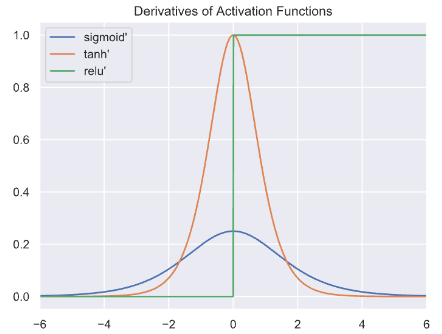
\includegraphics[width=0.3\linewidth]{img/RNN/derivatives.png}
              \caption{Solution 1: Activation function. ReLU prevents $f'$, to
                  shrink gradients when $x > 0$}
              \label{fig:activation}
          \end{figure}
    \item \textbf{Initialization}: We can initialize weights as an identity matrix
          and biases as 0, though this approach is not universally effective.
    \item \textbf{Architecture}: Modifying the architecture by incorporating gates
          to regulate the flow of information (e.g., as seen in ResNet) often
          proves to be the most robust solution.
\end{itemize}
\section{Gated RNNs}
In standard RNNs Figure \ref{fig:sRNN}, repeating modules contain a simple
computation node.
\begin{figure}[!ht]
    \centering
    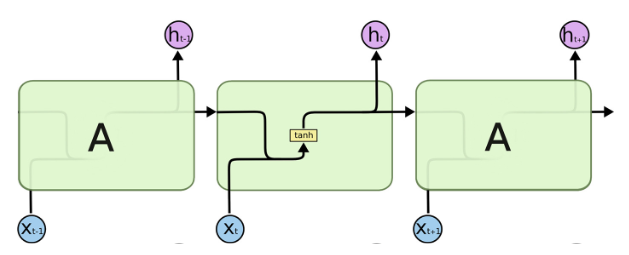
\includegraphics[width=0.5\linewidth]{img/RNN/sRNN.png}
    \caption{Standard RNN representation}
    \label{fig:sRNN}
\end{figure}

The most effective sequence models used in practical applications are called
\textbf{gated RNNs}. These include the \textbf{long short-term memory} (LSTM) and
networks based on the \textbf{gated recurrent unit} (GRU). Gated RNNs are based
on the idea of creating paths through time that have derivatives that neither
vanish nor explode.

\subsection{Long Short-Term Memory LSTM}
The clever idea of introducing self-loops to produce paths where the gradient can
flow for long durations is a core contribution of the initial \textbf{long short-
    term memory} (LSTM) model. A crucial addition has been to make the weight on
this self-loop conditioned on the context, rather than fixed. By making the weight
of this self-loop gated (controlled by another hidden unit), the time scale of
integration can be changed dynamically.

In this case, we mean that even for an LSTM with fixed parameters, the time scale
of integration can change based on the input sequence, because the time constants
are output by the model itself.

The LSTM block diagram is illustrated in Figure \ref{fig:lstm}. Instead of a unit
that simply applies an element-wise nonlinearity to the affine transformation of
inputs and recurrent units, LSTM recurrent networks have “LSTM cells” that have
an internal recurrence (a self-loop), in addition to the outer recurrence of the
RNN. Each cell has the same inputs and outputs as an ordinary recurrent network,
but also has more parameters and a system of gating units that controls the flow
of information.

\begin{figure}[!ht]
    \centering
    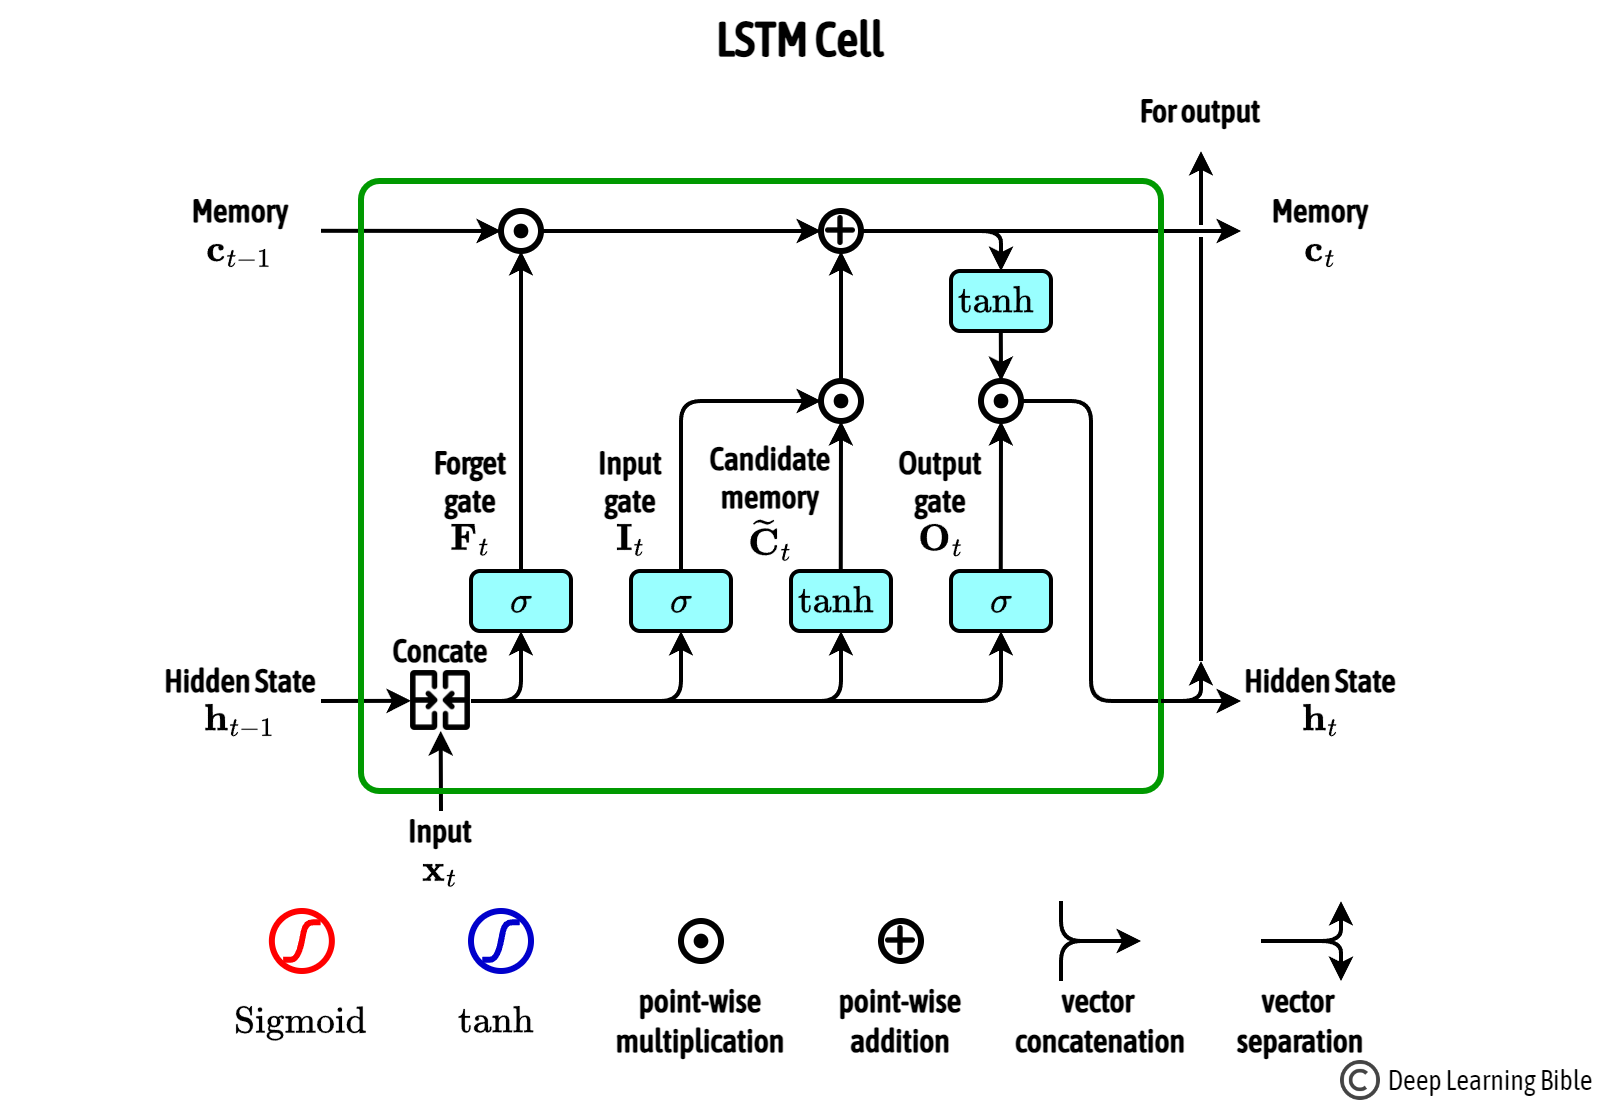
\includegraphics[width=0.5\linewidth]{img/RNN/LSTM_2.png}
    \caption{LSTM cell}
    \label{fig:lstm}
\end{figure}

LSTM cells are organized as follows:
\begin{itemize}
    \item \textbf{Forget gate}: decides which information from long term memory
          be kept or discarded and this is done by multiplying the incoming long
          term memory by a forget vector generated by the current input and
          incoming short memory:
          \begin{equation*}
              f_t = \sigma(W_f \cdot [h^{(t - 1)}, x^{(t)}] + b_f)
          \end{equation*}
    \item \textbf{Input gate}: decides what information will be stored in long
          term memory. It only works with the information from the current input
          and short term memory from the previous step. At this gate, it filters
          out the information from variables that are not useful. First, determine
          which entries in the cell state to update by computing $0 - 1$ sigmoid
          output:
          \begin{equation*}
              i^{(t)} = \sigma(W_i \cdot [h^{(t - 1)}, x^{(t)}] + b_i)
          \end{equation*}
          Then determine what amount to add/subtract from these entries by computing
          a tanh output (valued $-1$ to $1$) function of the input and hidden state:
          \begin{equation*}
              \tilde{C}^{(t)} = \tanh(W_c \cdot [h^{(t - 1)}, x^{(t)}] + b_c)
          \end{equation*}
    \item \textbf{Output gate}: will take the current input, the previous short
          term memory and newly computed long term memory to produce new short
          term memory which will be passed on to the cell in the next time step.
          Hidden state is updated based on a \textit{filtered} version of the
          cell state, scaled to $- 1$ to $1$ using tanh. Output gate computes a
          sigmoid function of the input and previous hidden state to determine
          which elements of the cell state to output:
          \begin{equation*}
              h^{(t)} = \sigma(W_o \cdot [h^{(t - 1)}, x^{(t)}] + b_o) \cdot \tanh C^{(t)}
          \end{equation*}
\end{itemize}

The previous state is multiplied by the forget gate and then added to the fraction
of the new candidate allowed by the input gate:
\begin{equation}
    C^{(t)} = f^{(t)} \cdot C^{(t - 1)} + i^{(t)} \cdot \tilde{C}^{(t)}
\end{equation}

\begin{figure}[!ht]
    \centering
    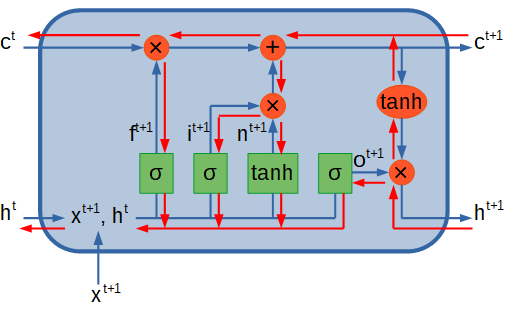
\includegraphics[width=0.45\linewidth]{img/RNN/backprop.png}
    \caption{Backpropagation through time with uninterrupted gradient flow}
    \label{fig:RNNBack}
\end{figure}
\subsection{GRU}
To solve the problem faced by standard RNN, GRU incorporates the two gate operating
mechanisms called \textbf{Update gate} and \textbf{Reset gate}. In particular,
it uses fewer gates than LSTM by combining forget and input gates into update gates
and eliminates cell state vector. This architecture has significant less number
of parameters so it is faster than the other.

\begin{figure}[!ht]
    \centering
    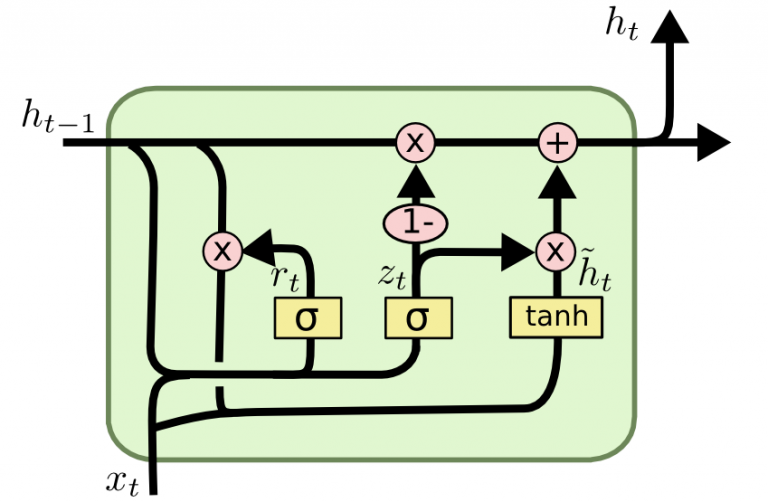
\includegraphics[width=0.45\linewidth]{img/RNN/GRU.png}
    \caption{GRU cell}
    \label{fig:gru}
\end{figure}

GRU cells are organized as follows:
\begin{itemize}
    \item \textbf{Update Gate}: is responsible for determining the amount of previous
          information that needs to pass along the next state. This is really
          powerful because the model can decide to copy all the information from
          the past and eliminate the risk of vanishing gradient;
    \item \textbf{Reset Gate}: it stores relevant information from the past time
          step into new memory content. Then it multiplies the input vector and
          hidden state with their weights. Next, it calculates element-wise
          multiplication between the reset gate and previously hidden state
          multiple. After summing up the above steps the non-linear activation
          function is applied and the next sequence is generated.
\end{itemize}
\chapter{Generative Adversarial Networks}
Many generative models are based on the idea of using a differentiable generator network. The model 
transforms samples of latent variables $z$ to samples $x$ or to distributions over samples $x$ using a 
differentiable function $g(z; \theta^{(g)})$, which is typically represented by a neural network. This 
model class includes \textbf{variational autoencoders}, which pair the generator net with an inference 
net; \textbf{generative adversarial networks} (GAN), which pair the generator network with a discriminator 
network; and techniques that train generator networks in isolation.

Generator networks are essentially just parametrized computational procedures for generating samples, 
where the architecture provides the family of possible distributions to sample from and the parameters 
select a distribution from within that family.

The goal of this model is to generate something starting from random noise. In order to do this, we want 
to create a model that is capable \textbf{to learn to sample} the distribution of the training set. 
Usually, this models are unsupervised because they do not use a labels. 

Its possible to create model that are able to generate a new sample based on some condition, for examples 
generating a new instance starting from a given label. Moreover, this models can be use for \textit{image 
    to image translation}. In this case we solve task like given a black\&white image and we want to 
generate the colored image. This feature makes these models very useful for performing computer vision 
tasks such as: increasing data, improving image, etc$\dots$

In order to build a generative model we need two main components:
\begin{itemize}
    \item The first is to define an architecture that allows a new sample to be generated.
    \item The second is to define the correct loss function. 
\end{itemize}
So we want to learn to sample, so $x \sim p_{data}$ should be $x_{gen}\sim p_{model}$, such manner that $p_{data} \equiv p_{model}$.
\section{Generator architecture}
During this course, we have already explored a type of neural network capable of generating data: the 
\textit{autoencoder}. Specifically, by isolating the decoder component and sampling from the latent space,
we can generate novel examples.

Up to this point we have only seen architectures that allow to reduce the size of the images (CNN). We
want to see how we can use these architectures to upsample a noise distribution. We start from a 
convolution like the one shown in figure \ref{fig:reg-conv}

\begin{figure}[!ht]
    \centering
    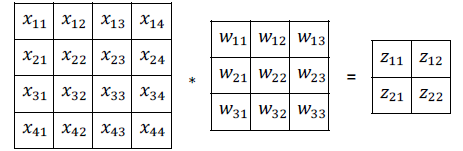
\includegraphics[width=0.5\linewidth]{img/GAN/RegularConv.png}
    \caption{Regular convolution stride 1, pad 0}
    \label{fig:reg-conv}
\end{figure}

We can rewrite this operation in a matrix form figure \ref{fig:conmat}.

\begin{figure}[!ht]
    \centering
    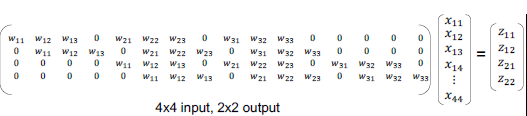
\includegraphics[width=0.5\linewidth]{img/GAN/matrix-vector.png}
    \caption{Matrix form}
    \label{fig:conmat}
\end{figure}

From here we realize that we can increase the size if we multiply our result by the transposition of the 
filter figure \ref{fig:traConv}. It is necessary to note that this operation does not correspond to the inverse of the original convolution.

\begin{figure}[!ht]
    \centering
    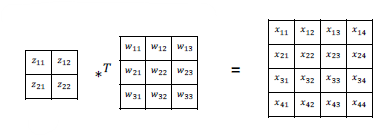
\includegraphics[width=0.5\linewidth]{img/GAN/transposeConv.png}
    \caption{Caption}
    \label{fig:traConv}
\end{figure}

The figure \ref{fig:TConvRes} shows the result of this operation at the graphic level.

\begin{figure}[!ht]
    \centering
    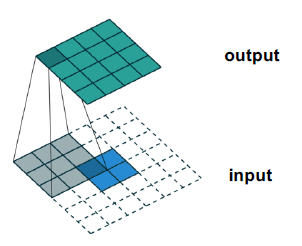
\includegraphics[width=0.5\linewidth]{img/GAN/results.png}
    \caption{Caption}
    \label{fig:TConvRes}
\end{figure}

Generative adversarial networks are based on a game theoretic scenario in which the generator network must 
compete against an adversary. The generator network directly produces samples $x = g(z; \theta^{(g)})$. 
Its adversary, the \textbf{discriminator network}, attempts to distinguish between samples drawn from the 
training data and samples drawn from the generator. The discriminator emits a probability value given by 
$d(x; \theta^{(d)})$, indicating the probability that $x$ is a real training example rather than a fake 
sample drawn from the model.
\section{Define the loss function}
The simplest way to formulate learning in generative adversarial networks is as a zero-sum game, in which 
a function $v(\theta^{(g)}, \theta^{(d)})$ determines the payoff of the discriminator. The generator 
receives $- v(\theta^{(g)}, \theta^{(d)})$ as its own payoff. During learning, each player attempts to 
maximize its own payoff, so that at convergence:
\begin{equation}
    g^\ast = \arg \min_{g} \max_{d} v(g, d)
\end{equation}
With this approach we are training the generator and the discriminator jointly in a \textbf{minimax game}, where 
both need to get better and better to improve the generation quality.

The default choice for $v$ is:
\begin{equation}
    V(\theta^{(g)}, \theta^{(d)}) = \mathbb{E}_{x \sim p_{data}} \log d(x) + \mathbb{E}_{z \sim p_{model}} \log(1 - d(g(z)))
\end{equation}
This drives the discriminator to attempt to learn to correctly classify samples as real or fake, in 
other words the discriminator wants to maximize:
\begin{equation*}
    d^\ast = \arg \max_d V(g,d)
\end{equation*}
Simultaneously, the generator attempts to fool the classifier into believing its samples are real:
\begin{equation*}
    G^\ast = \arg \min_G V(G,D)
\end{equation*}

In general, simultaneous gradient descent on two players’ costs is not guaranteed to reach an equilibrium. 
Note that the equilibria for a minimax game are not local minima of $v$. Instead, they are points that are 
simultaneously minima for both players’ costs. This means that they are saddle points of $v$ that are 
local minima with respect to the first player’s parameters and local maxima with respect to the second 
player's parameters.

The training process therefore consists of alternating between:
\begin{itemize}
    \item Gradient ascent on discriminator: 
        \begin{equation}
            D^\ast = \arg \max_D V(G,D)
        \end{equation}
    \item Gradient descent on generator (minimize log-probability of discriminator being right):
        \begin{equation}
            G^\ast = \arg \min_G V(G,D) = \arg \min_G \mathbb{E}_{z\sim p_{gen}} \log(1-D(G(z)))  =  \arg \max_G \mathbb{E}_{z\sim p_{gen}} \log(D(G(z)))
        \end{equation}
\end{itemize}

\begin{figure}[!ht]
    \centering
    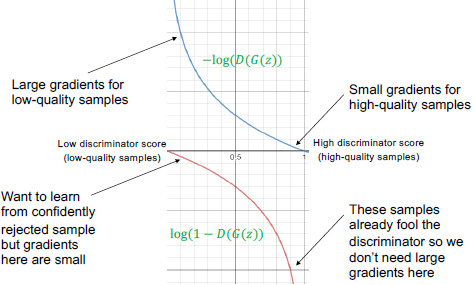
\includegraphics[width=0.5\linewidth]{img/GAN/loss.png}
    \caption{Loss function}
    \label{fig:enter-label}
\end{figure}
 
In the original version the loss of the generator $G$ learns fewer from initial image generated, but in
this moment we want to learn more, the opposite thing happen for higher value of the discriminator and
this isn't useful. So we rewrite the loss function using  $1 - \log(D(G(z)))$ in order to learn more at
the starting of the training.

The process for updating the generator increase $D(G(z))$ requires back-propagating through the composed
generator-discriminator network i.e., the discriminator cannot be a black box. The generator is exposed to 
real data only via the output of the discriminator and its gradients.

Stabilization of GAN learning remains an open problem. Fortunately, GAN learning performs well when the 
model architecture and hyperparameters are carefully selected.

The GAN learning problem can also be simplified by breaking the generation process into many levels of 
detail. It is possible to train conditional GANs that learn to sample from a distribution $p(x | y)$ 
rather than simply sampling from a marginal distribution $p(x)$. 

Also, we have the problem of \textbf{mode collapse} where the generator ends up modeling only a small
subset of the training data.

Make sure discriminator provides good gradients to the generator even when it can confidently reject all 
generator samples. Use non-saturating generator. Smooth discriminator targets for “real” data, e.g., use
target value 0.9 instead of 1 when training discriminator

\section{Evaluating Generative Models}
Generative modeling is different from normal model because changes in preprocessing, even very small and 
subtle ones, are completely unacceptable. Any change to the input data changes the distribution to be 
captured and fundamentally alters the task.

Because being able to generate realistic samples from the data distribution is one of the goals of a 
generative model, practitioners often evaluate generative models by visually inspecting the samples. 
Unfortunately, it is possible for a very poor probabilistic model to produce very good samples. Imagine a 
generative model trained on images of dogs and cats that simply learns to reproduce the training images of 
dogs. Such a model has clearly overfit, because it does not produces images that were not in the training 
set, but it has also underfit, because it assigns no probability to the training images of cats. Yet a 
human observer would judge each individual image of a dog to be high quality. In more realistic settings, 
a generative model trained on data with tens of thousands of modes may ignore a small number of modes, and 
a human observer would not easily be able to inspect or remember  enough images to detect the missing 
variation.

Since the visual quality of samples is not a reliable guide, we often also evaluate the log-likelihood 
that the model assigns to the test data, when this is computationally feasible. Unfortunately, in some 
cases the likelihood seems not to measure any attribute of the model that we really care about.

The fact that there are many different uses of generative models the choice of metric must match the 
intended use of the model.


We pass from discriminator to update a generator because we don't know which loss put in output to generator.
\chapter{Federated Learning}
The standard setting in Machine Learning (ML) considers a centralized dataset
processed in a tightly integrated system, but in the real world data is often
decentralized across many parties. One challenge is that collecting these data
at a single point is not always feasible for various reasons. Transmitting the
data might be prohibitively expensive, such as when dealing with large volumes
of data, or it may be constrained by the limited bandwidth or power capacity of
wireless devices.

Another challenge is that the data might be believed too sensitive. In recent
years, there has been increasing public awareness and stricter regulations
concerning data privacy. Additionally, maintaining control over data can offer a
competitive edge in both business and research contexts.

One possible solution could be to create a separate model for each data source,
utilizing the data available locally. However, this approach has significant
drawbacks. The amount of data at each source may be too limited, leading to
overfitting or decisions that lack statistical significance. Moreover, the
local dataset may fail to accurately represent the overall target distribution,
further compromising the model's effectiveness.

\textbf{Federated Learning} (FL) aims to collaboratively train a ML model while
keeping the data decentralized. The methodology for implementing federated
learning is as follows:
\begin{enumerate}
    \item The server initialize the model weights and send a copy to all the parties;
    \item Each party make an update using its local dataset;
    \item Parties share local updates for aggregation;
    \item Server aggregates updates and send back to parties;
    \item Parties update their copy of the model and iterate.
\end{enumerate}

We would like the final model to be as good as the centralized solution (ideally),
or at least better than what each party can learn on its own.

\begin{note}
    The assumption is that starting from the weights we cannot obtain the data,
    otherwise we could have just send the data.
\end{note}

More broadly, we can categorize federated learning (FL) into different
classifications. The first classification differentiates between:
\begin{itemize}
    \item \textbf{Cross-device FL}: this scenario involves a large number of
          participants, each possessing a small dataset. Additionally, it is
          important to account for the fact that some participants may not always
          be reachable, and some may have malicious intentions, posing further
          challenges.
    \item \textbf{Cross-silo}: in this scenario we have a limited number of parties
          with medium large dataset. Parties are always available and are
          typically honest.
\end{itemize}

Another type of classification is:
\begin{itemize}
    \item \textbf{Server orchestrated FL}: where we have a server that performs
          global coordination and aggregation. The server is the bottleneck and
          a single point of failure.
    \item \textbf{Device-to-device communication}: peer to peer communication
          between the parties. This approach can scale better.
\end{itemize}

\section{Distributed Learning}
A different training paradigm is \textbf{distributed learning}. In this approach,
unlike federated learning (FL), the data is initially centralized and then distributed
later to accelerate model training. The key distinction from FL lies in how the
data is distributed: in distributed learning, the data is typically distributed
uniformly at random across workers under controlled conditions.

In contrast, FL involves data that is naturally distributed and generated locally.
This data is often not independent and identically distributed (non-i.i.d.) and
is usually imbalanced. FL also introduces additional challenges that span various
fields of computer science, such as enforcing privacy constraints, addressing
the potentially limited reliability and availability of participants, ensuring
robustness against malicious actors, and more.
\section{Baseline algorithm: FedAvg}
Let's start by introducing some notation. Let's consider a set of $K$ parts
(clients). Each part $k$ holds a data set $\mathcal{D}_k$ composed of $n_k$
instances. Let $\mathcal{D} = \mathcal{D}_1 \cup \dots \cup \mathcal{D}_K$ be the
total dataset and $n = \sum_k n_k$ the total number of instance.

In this situation, we want to solve the problems of the form:
\begin{equation}
    \min_{\theta \in \mathbb{R}^p} F(\theta; \mathcal{D})
\end{equation}
where:
\begin{equation}
    F(\theta; \mathcal{D}) = \sum_{k = 1}^K \frac{n_k}{n} F_k(\theta; \mathcal{D}_k) \,\,\, \text{ and }
    \,\,\, F_k(\theta; \mathcal{D}_k) = \sum_{d \in \mathcal{D}_k} f(\theta; d)
\end{equation}
where $\theta \in \mathbb{R}^p$ are model parameters such as neural network weights.

\begin{multicols}{2}
    \noindent
    \textbf{Algorithm: FedAvg (server-side)} \\
    \textbf{Parameters:} client sampling rate $\rho$ \\
    \begin{algorithmic}[1]
        \State Initialize $\theta$
        \For{each round $t = 0, 1, \dots$}
        \State $S_t \gets$ random set of $m = \lceil \rho K \rceil$ clients
        \For{each client $k \in S_t$ in parallel}
        \State $\theta_k \gets \text{ClientUpdate}(k, \theta)$
        \EndFor
        \State $\theta \gets \sum_{k \in S_t} \frac{n_k}{n} \theta_k$
        \EndFor
    \end{algorithmic}

    \vfill

    \columnbreak

    \noindent
    \textbf{Algorithm: ClientUpdate($k, \theta$)} \\
    \textbf{Parameters:} batch size $B$, number of local steps $L$, learning rate $\eta$ \\
    \begin{algorithmic}[1]
        \For{each local step $l = 1, \dots, L$}
        \State $B \gets$ mini-batch of $b$ examples from $\mathcal{D}_k$
        \State $\theta \gets \theta - \frac{\eta}{B} \sum_{d \in B} \nabla \ell(\theta; d)$
        \EndFor
        \State \textbf{send} $\theta$ to server
    \end{algorithmic}
\end{multicols}

\textbf{Notes:}
\begin{itemize}
    \item For $L = 1$ and $\rho = 1$, it is equivalent to classic parallel SGD:
          updates are aggregated, and the model is synchronized at each step.
    \item For $L > 1$, each client performs multiple local SGD steps before communicating.
\end{itemize}

\textbf{FedAvg} with $L > 1$ allows to reduce the number of communication rounds,
which is often the bottleneck in FL. It empirically achieves better generalization
than parallel SGD with large mini-batch. Convergence to the optimal model can be
guaranteed for i.i.d. data, but issues arise in strongly non-i.i.d. cases.

Learning from non-i.i.d. data is difficult/slow because each party wants the model
to go in a particular direction. If data distributions are very different, learning
a single model which performs well for all parties may require a very large number
of parameters.

Another direction to deal with non-i.i.d. data is thus to lift the requirement
that the learned model should be the same for all parties. Instead, we can allow
each party $k$ to learn a (potentially simpler) personalized model $\theta_k$
but design the objective so as to enforce some kind of collaboration.

Several strategies have been developed to manage the combination of this last
idea, including:
\begin{itemize}
    \item A first approach propose to regularize personalized models to their mean:
          \begin{equation}
              F(\theta_1, \dots, \theta_k; \mathcal{D}) = \frac{1}{K} \sum_{k = 1}^K F_k(\theta_k; \mathcal{D}) + \frac{\lambda}{2 \cdot K} \sum_{k = 1}^K \left\|\theta_k - \frac{1}{K} \sum_{i = i}^K \theta_i\right\|
          \end{equation}
    \item Another approach, inspired by \textbf{meta-learning}, propose to learn
          a global model which easily adapts to each party:
          \begin{equation}
              F(\theta; \mathcal{D}) = \frac{1}{K} \sum_{k = 1}^K F_k(\theta - \alpha \cdot \nabla F_k(\theta); \mathcal{D})
          \end{equation}
\end{itemize}

We can remove outliers using median at the place of mean.
\chapter{Transformers}
\textbf{Transformer} were initially targeted at natural language processing (NLP)
problems, where the network input is a series of high-dimensional embeddings
representing words or word fragments. This architecture was designed with the goal
of processing this text into a representation suitable for downstream tasks.

We can also encounter different problems such as:
\begin{itemize}
    \item The encoded input can be very large. Assuming a 1024-d embedding and
          body of text that have 100s/1000s of words, a fully connected neural
          network is impractical because we have $100 \times 1024 = 102400$ as
          input length;
    \item Each input is of different length and Feed Forward Neural Networks are
          impracticable;
    \item Statistics are similar at every position;
    \item The language is fundamentally ambiguous.
\end{itemize}

Most of these problems are derived by NLP problems.
\section{Dot-product self attention}
Considering the issues just presented, we want to design a network that is able
to process text and can:
\begin{enumerate}
    \item Use parameter sharing to cope with long input passages of differing
          lengths;
    \item Contain connections between word representations that depend on the
          words themselves.
\end{enumerate}
The transformer acquires both properties by using \textbf{Dot-Product Self-Attention}.
This mechanism is shown in Figure \ref{fig:sa}.

\begin{figure}[!ht]
    \centering
    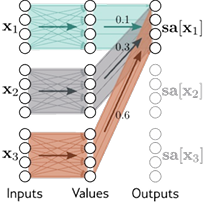
\includegraphics[width=0.3\linewidth]{img/transformer/selfattention.png}
    \caption{Dot-Product Self-Attention mechanism}
    \label{fig:sa}
\end{figure}

While a standard NN layer $f[x]$ takes a $D\times 1$ input $x$ and applies a
linear transformation followed by a non-linear activation function $a[\cdot]$:
\begin{equation*}
    f[x] = a[\beta + \Omega x]
\end{equation*}
where $\beta$ contains the biases and $\Omega$ contains weights. A self-attention
block $sa[\cdot]$ takes $N$ inputs $x_n$, each of dimension $D \times 1$, and
returns $N$ output vectors of the same size. In the context of NLP, each $x_n$
will represent a word or a word fragment of a sentence.

Let's go into more detail. First, a set of \textbf{values} are computed for each
input:
\begin{equation}
    v_n = \beta_v + \Omega_v \cdot x_n
\end{equation}
where $\beta_v$ contains the biases and $\Omega_v$ contains the weights. Then the
$n$-th output $sa[x_n]$ is a weighted sum of all the values $v_n$:
\begin{equation}
    sa[x_n] = \sum_{m = 1}^N a[x_m, x_n] \cdot v_m
\end{equation}
The scalar weight $a[x_m, x_n]$ is the \textbf{attention} that input $x_n$ pays
to input $x_m$. The $N$ weights $a[\cdot, x_n]$ are non-negative and sum to one.

Self-attention can be understood as a mechanism that routes the values in different
proportions to construct each output.

To compute the values, the same weights $\Omega_v$ ($D \times D$) and biases
$\beta_v$ ($D \times 1$) are applied to each input $x_n$ ($D \times 1$):
\begin{equation}
    v_n = \beta_v + \Omega_v \cdot x_n
\end{equation}
This computation scales linearly with the sequence length $N$, so it requires less
parameters than a fully connected neural network connecting all $DN$ inputs to
the $DN$ outputs.

The value computation can thus be viewed as a sparse matrix multiplication (see
Figure \ref{fig:valuesComputation}) with shared parameters.
\begin{figure}[!ht]
    \centering
    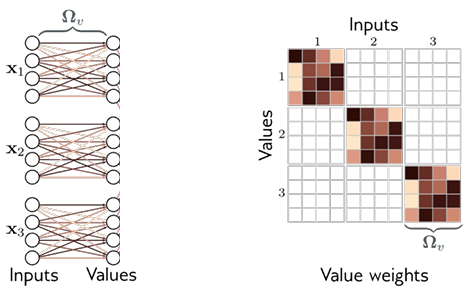
\includegraphics[width=0.5\linewidth]{img/transformer/values.png}
    \caption{Values computation in self-attention using shared parameters}
    \label{fig:valuesComputation}
\end{figure}

The attention weights $a[x_m, x_n]$ combine the values from different inputs. They
are also sparse (Figure \ref{fig:attention}), since there is only one weight for
each ordered pair of inputs $(x_m, x_n)$regardless of the size of these inputs.

\begin{figure}[!ht]
    \centering
    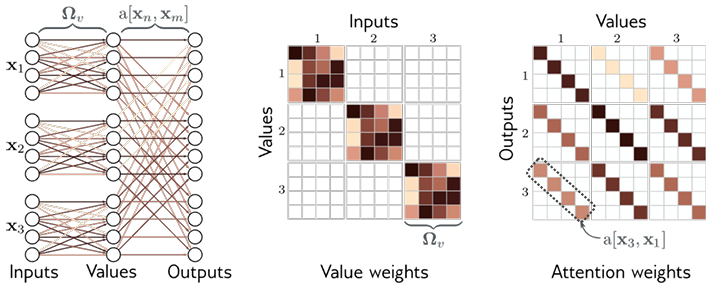
\includegraphics[width=0.6\linewidth]{img/transformer/attention.png}
    \caption{Attention}
    \label{fig:attention}
\end{figure}

The number of attention weights has a quadratic dependence on the sequence length
$N$ but it is independent of the length $D$ of each input $x_n$.

Through this process, you get the same output as that from two-chained linear
transformations:
\begin{itemize}
    \item The value vectors are computed independently from each input;
    \item and these vectors are linearly combined by the attention weights.
\end{itemize}

However, the overall self-attention is non-linear because the attention weights
are themselves non-linear functions of the input. This is an example of a
\textbf{hypernetwork}, where one network branch computes the weights of another
branch.

To compute the \textit{attention}, we apply two more linear transformations to
the inputs:
\begin{equation}
    q_n = \beta_q + \Omega_q \cdot x_n \,\,\, \land \,\,\, k_n = \beta_k + \Omega_k \cdot x_n
\end{equation}
where $q_n$ and $k_n$ are referred to as the \textbf{queries} and the \textbf{keys}.

We then compute dot products between the queries and the keys followed by a softmax:
\begin{equation}
    a[x_m, x_n] = softmax_m [k_\ast^T, q_n] = \frac{\exp[k_\ast^T, q_n]}{\sum_{m' = 1}^N \exp[k_\ast^T, q_n]}
\end{equation}
so, for each $x_n$ they are positive and sum to one and these is the method to apply
non linearity on attention.

The names \textit{queries} and \textit{keys} have the following interpretation:
\begin{itemize}
    \item The dot-product operation returns a measure of similarity between its
          inputs, so the weights $a[x_\ast, x_n]$ depend on the relative similarities
          between each query and the keys;
    \item The softmax function means that we can think of the key vectors as
          \textit{competing} with one another to contribute to the final result.
\end{itemize}
The queries and keys must have the same dimensions.

However, these can differ from the dimension of the values, which is usually the
same size as the input, so that the representation does not change size.

This mechanism fulfills the initial requirements:
\begin{enumerate}
    \item There is a single shared set of parameters $\phi = \{\beta_v, \Omega_v,
              \beta_q, \Omega_q, \beta_k, \Omega_k\}$. This is independent of the
          number of inputs $N$, so the networks can be applied to difference
          sequence lengths;
    \item There are connections between the inputs (words), and the strength of
          these connections depends on the inputs themselves via the attention weights.
\end{enumerate}

This can be written in a compact form if the $N$ inputs $x_n$ form the columns of
the $D \times N$ matrix $X$. The values, queries, and keys can be computed as:
\begin{align*}
    V[X] = \beta_v \cdot 1^T + \Omega_v \cdot X \\
    Q[X] = \beta_q \cdot 1^T + \Omega_q \cdot X \\
    K[X] = \beta_k \cdot 1^T + \Omega_k \cdot X
\end{align*}
The self-attention computation is then:
\begin{equation}
    sa[X] = V[X] \cdot softmax[K[X]^T, Q[X]]
\end{equation}
where softmax is independently applied on the columns of its input.

Since the dot-product in the attention calculation can result in large magnitudes,
it pushes the arguments of the softmax function into a region where the largest
value dominates entirely. This causes small changes to the softmax inputs to
have minimal impact on the output, making the model harder to train.

To mitigate this, the dot products are scaled by the square root of the size of
the query $D_q$ and key $D_k$, which corresponds to the number of rows in $\Omega_q$
and $\Omega_k$ as the query and key dimensions must be the same.
\begin{equation}
    sa[X] = V \cdot softmax\left[\frac{K^T \cdot Q}{\sqrt{D_q}}\right]
\end{equation}

\section{Positional encoding}
The self-attention mechanism discards important information, in fact, the computation
is the same regardless of the order of the inputs. However, the order is important
when the inputs correspond to the words in a sentence. There are two main approaches
to incorporating position information:
\begin{itemize}
    \item \textbf{Absolute position embeddings};
    \item \textbf{Relative position embeddings}.
\end{itemize}
\subsection{Absolute position embeddings}
This method consists of adding a $\Pi$ matrix to the $X$ input. The purpose of
this matrix is to encode positional information. Each column of $\Pi$ is unique
and contains information about the absolute position in the input sequence.

The matrix that is usually used for this purpose can be handcrafted or learned in
the model training phase. Typically, this matrix is added to the model's input.
Alternatively, since the outputs of the self-attention blocks have the same dimensions
as the input, the matrix can be added after each layer.

\begin{note}
    Sometimes it is added to $X$ in the computation of the queries and keys but
    not to the values.
\end{note}

\subsection{Relative position embeddings}
In this case, we are considering a situation where the input to a self-attention
mechanism may be an entire sentence, many sentences, or just a fragment of a sentence,
and the absolute position of a word is much less important than the relative
position between two inputs. Of course, this can be recovered if the system knows
the absolute position of both, but relative position embeddings encode this
information directly. Each element of the attention matrix corresponds to a
particular offset between query position $a$ and key position $b$.

Relative position embeddings learn a parameter $\pi_{a, b}$, for each offset and
use this to modify the attention matrix by adding these values, multiplying by them,
or using them to alter the attention matrix in some other way.
\section{Multiple heads self attention}
In the most used architectures, multiple self-attention mechanisms are used in
parallel, and this is known as \textbf{Multi-Head Self-Attention}. If we now
consider the fact of having $H$ self-attention blocks, we have that the different
sets of values, keys and queries are calculated as:
\begin{align*}
    V_h[X] = \beta_{vh} \cdot 1^T + \Omega_{vh} \cdot X \\
    Q_h[X] = \beta_{qh} \cdot 1^T + \Omega_{qh} \cdot X \\
    K_h[X] = \beta_{kh} \cdot 1^T + \Omega_{kh} \cdot X
\end{align*}
Then, the $h-$th self-attention mechanism or \textbf{head} can be written as:
\begin{equation}
    sa_h[X] = V_h \cdot softmax\left[\frac{K_h^T \cdot Q_h}{\sqrt{D_q}}\right]
\end{equation}
where we have different parameters for each head.

Typically, if the dimension of the inputs $x_m$ is $D$ and there are $H$ heads,
the values, queries, and keys will all be of size $D / H$ as this allows for an
efficient implementation. The outputs of these self-attention mechanisms are then
vertically concatenated, and another linear transform $\Omega_c$ is applied to
combine them. An example with $H = 2$ is shown in Figure \ref{fig:multiHead}.
The output of the multi-head self-attention mechanism is then:
\begin{equation}
    Mhsa[X] = \Omega_c[sa_1[X]^T, sa_2[X]^T, \dots, sa_H[X]^T]
\end{equation}
\begin{figure}[!ht]
    \centering
    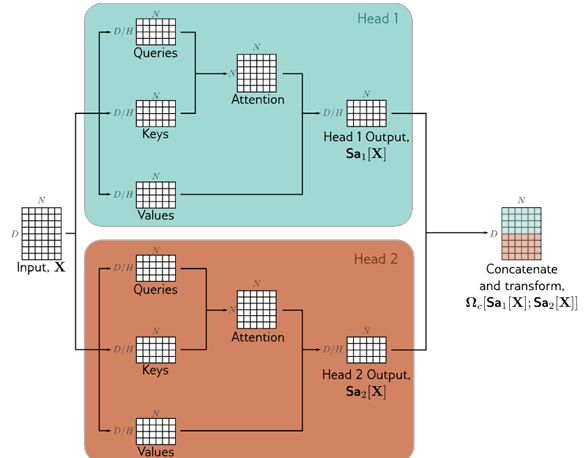
\includegraphics[width=0.5\linewidth]{img/transformer/multihead.png}
    \caption{Multi-Head Self-Attention example with $H = 2$}
    \label{fig:multiHead}
\end{figure}

This last transformation is useful because it allows to bring the weights of the
different heads in the same range. In addition, if necessary, this combination
can be used to limit a head that provides wrong data in output by setting it to
zero.

Multiple heads seem to be necessary to make the transformer work well. It has
been speculated that they make the self-attention network more robust to bad
initializations.

\section{Transformer Layers}
All the components we have defined so far serve as a basis for defining the
\textbf{Transformer Layer}. This is the basic building block of the transformer
architecture. The structure of a Transformer Layer is shown in Figure \ref{fig:transformerLayers}.

\begin{figure}[!ht]
    \centering
    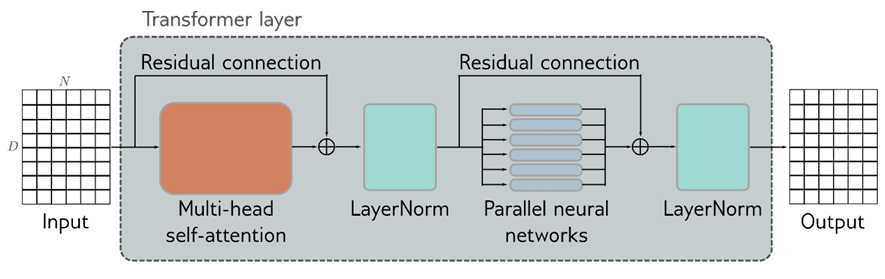
\includegraphics[width=0.5\linewidth]{img/transformer/transformerlayers.png}
    \caption{Transformer Layers}
    \label{fig:transformerLayers}
\end{figure}

Transformer Layer consists of a multi-head self-attention unit, which allows the
word representations to interact with each other, followed by a fully connected
network $mlp[x_\ast]$ that operates separately on each word. Both units are
residual networks.

In addition, it is typical to add a \textbf{LayerNorm} operation after both the
Self-Attention and Fully Connected Networks.

Architecture that are now used in practice are more complex in the sense that
they have more than one layer of self-attention and fully connected networks.

\section{NLP pipeline}
A typical NLP pipeline begins with a \textbf{tokenizer}, which splits text into
a vocabulary of smaller constituent units (tokens) that the subsequent network
can process. These tokens often represent words, but several challenges arise:
\begin{itemize}
    \item Inevitably, some words (e.g., names) will not be present in the vocabulary;
    \item Handling punctuation can be unclear, yet crucial. For example, if a
          sentence ends with a question mark, this information must be encoded;
    \item The vocabulary would require separate tokens for different forms of the
          same word (e.g., variations with different suffixes), with no mechanism
          to clarify that these variations are related.
\end{itemize}

Each of these tokens is mapped to a learned embedding. These embeddings are then
passed through a series of transformer layers. We will now examine each of these
stages in detail.

In practice, a compromise between letters and full words is employed. The final
vocabulary includes both common words and word fragments, which can be combined
to represent larger and less frequent words. This vocabulary is typically generated
using a sub-word tokenizer, such as byte pair encoding (BPE), which greedily merges
frequently occurring substrings based on their frequency.

Each token in the vocabulary $\mathcal{V}$ is consistently mapped to a corresponding
word embedding, ensuring that the same token always maps to the same embedding.

To accomplish this, the $N$ input tokens are represented in the matrix $T$, with
dimensions $|V| \times N$. Each column of $T$ corresponds to a token, where the
$n$-th column represents the $n$-th token as a one-hot vector of size $|V| \times 1$.

The embeddings for the entire vocabulary are stored in a matrix $\Omega_e$, with
dimensions $D \times |V|$. The input embeddings are computed as $X = \Omega_e \cdot T$,
where $\Omega_e$ is learned like any other parameter of the network.

A typical embedding size $D$ is 1024, and a typical vocabulary size $|V|$ is 30,000.
As a result, even before the main network processes the data, the matrix $\Omega_e$
contains a large number of parameters to learn.

Finally, the embedding matrix $X$, which represents the text, is passed through
a series of transformer layers, forming what is known as a transformer model.


There are three types of transformer models:
\begin{enumerate}
    \item \textbf{Encoders}: An encoder transforms text embeddings into representations
          that support a variety of tasks. \textbf{BERT} (Bidirectional Encoder
          Representations from Transformers) is an example of an encoder model
          with a vocabulary of 30,000 tokens. Input tokens are mapped to 1,024-dimensional
          word embeddings and processed through 24 transformer layers, each
          containing a self-attention mechanism with 16 heads. Each head computes
          queries, keys, and values with a dimension of 64. Encoder models like
          BERT employ transfer learning. During pretraining, the transformer's
          parameters are learned via self-supervision on a large text corpus. The
          pretraining objective is to capture general statistical knowledge of
          language through tasks such as predicting missing words in sentences.
          The learned text representations can then be fine-tuned for specific
          NLP tasks.
    \item \textbf{Decoders}: A decoder generates new tokens to extend an input
          text sequence. For example, \textbf{GPT-3} constructs an autoregressive
          language model, where the joint probability of a sequence of tokens
          $(t_1, t_2, \dots, t_N)$ is factored as:
          \begin{equation}
              P(t_1, t_2, \dots, t_N) = P(t_1) \cdot \prod_{n=2}^N P(t_n \mid t_1, \dots, t_{n-1})
          \end{equation}
          This autoregressive approach defines a probability distribution over
          text sequences, enabling the generation of new, coherent text. Given an
          input sequence, the model predicts a probability distribution over
          possible next tokens. The selected token is appended to the sequence and
          fed back into the model, repeating the process iteratively to generate
          text.
    \item \textbf{Encoder-Decoders}: Encoder-decoder models are designed for
          sequence-to-sequence tasks, such as \textbf{machine translation}, where
          text in one language is transformed into another. These models encode
          the input sequence into a latent representation and decode it into the
          target sequence.
\end{enumerate}
\chapter{Self-Supervised Learning}
The models trained from large-scale of data, such as the ImageNet dataset, are
widely used as the pre-trained models and fine-tuned for other tasks for two main
reasons:
\begin{itemize}
      \item The parameters learned from large-scale diverse datasets provide a
            good starting point, therefore, networks training on other tasks can
            converge faster;
      \item The network trained on large-scale datasets already learned the hierarchy
            features which can help to reduce over-fitting problem during the
            training of other tasks, especially when datasets of other tasks are
            small, or training labels are scarce.
\end{itemize}

With the sophisticated architectures and large-scale datasets, the performance
of DNNs keeps breaking the state-of-the-arts for many tasks. However, collection
and annotation of large-scale datasets are time-consuming and expensive.

To avoid time-consuming and expensive data annotations, many \textbf{self-supervised}
methods were proposed to learn visual features from large-scale unlabeled images
or videos without using any human annotations.

A popular solution is to propose various pretext tasks for networks to solve. The
networks can be trained by learning objective functions of the pretext tasks and
in the while the features are learned through this process. Thanks to the pretext
tasks, the data are labeled automatically.

The model created using this method can be used as a pre-trained model and applied
to the supervised downstream tasks to improve the performance.

Various pretext tasks have been proposed for self-supervised learning including
colorizing gray scale images, image inpainting, playing image jigsaw puzzle, etc.
The pretext tasks share two common properties:

\begin{itemize}
      \item Visual features of images or videos need to be captured by CNNs to
            solve the pretext tasks;
      \item The supervisory signal is generated from the data itself (self-supervision)
            by leveraging its structure.
\end{itemize}

During the self-supervised training phase, a predefined pretext task is designed
for CNNs to solve, and the pseudo labels for the pretext task are automatically
generated based on some attributes of data.

Then the CNN is trained to learn objective functions of the pretext task. As with
training on a labeled dataset, when trained with pretext tasks, the shallower
blocks of CNN focus on the low-level general features such as corners, edges, and
textures, while the deeper blocks focus on the high-level task-specific features
such as objects, scenes, and object parts. Therefore, CNNs trained with pretext
tasks can learn kernels that capture low-level features and high-level features
that are helpful for other downstream tasks.

After the self-supervised training is finished, the learned visual features can
be further transferred to downstream tasks as pre-trained models to improve
performance and overcome over-fitting.

The main advantage of self-supervised learning methods is that they can be easily
scaled to large-scale datasets with very low cost.

We now present the terminology that will be used during this section:
\begin{itemize}
      \item \textbf{Human-annotated label}: labels of data that are manually
            annotated by human workers.
      \item \textbf{Pretext Task}: pre-designed tasks for networks to solve, and
            visual features are learned by learning objective functions of pretext
            tasks. The pretext tasks can be predictive tasks, generative tasks,
            contrasting tasks, or a combination of them. The supervision signal
            for pretext tasks is generated from the data itself based on its structure.
      \item \textbf{Pseudo label}: The labels used in pretext task is referred as
            Pseudo labels which are generated based on the structure of data for
            pretext tasks.
      \item \textbf{Downstream Task}: CV applications that can be used to evaluate
            the quality of features learned by self-supervised learning. These
            applications can greatly benefit from the pre-trained models when training
            data are scarce. In general, human-annotated labels are needed to solve
            the downstream tasks. However, in some applications, the downstream task
            can be the same as the pretext task without using any human-annotated
            labels.
      \item \textbf{Supervised Learning}: refers to learning methods using data with
            fine-grained human annotated labels to train networks.
      \item \textbf{Semi-supervised Learning}: refers to learning methods using a
            small amount of labeled data in conjunction with a large amount of
            unlabeled data.
      \item \textbf{Weakly-supervised Learning}: refers to learning methods to learn
            with coarse-grained labels or inaccurate labels. The cost of obtaining
            weak supervision labels is generally much cheaper than fine-grained
            labels for supervised methods.
      \item \textbf{Unsupervised Learning}: refers to learning methods without using
            any human-annotated labels.
      \item \textbf{Self-supervised Learning}: refers to learning methods in which
            CNNs are explicitly trained with supervisory signals that are generated
            from the data itself (self-supervision) by leveraging its structure.
\end{itemize}

We can compare the performance of image feature training by evaluating the
classificator on the same dataset.
\begin{note}
      Self supervised learning add robustness to model.
\end{note}
\section{Learning visual features from pretexts tasks}
To relieve the burden of large-scale dataset annotation, a pretext task is generally
designed for networks to solve while pseudo labels for the pretext task are
automatically generated based on data attributes. Effective pretext tasks are
those ensuring that semantic features are learned through the process of accomplishing
the pretext tasks.

As we have seen before, there are different types of pretext task that can be used
to train a neural network with self supervised learning. We can classify them
into four categories as shown in Figure \ref{fig:SSL}.

\begin{figure}[!ht]
      \centering
      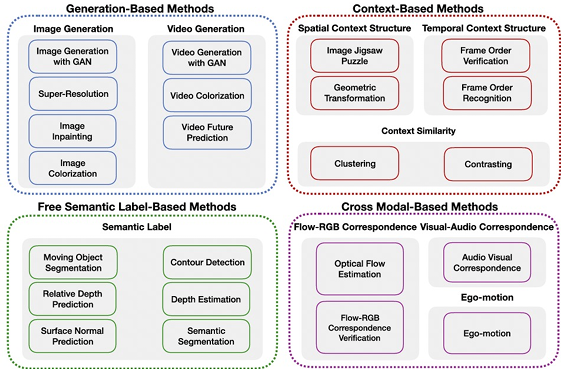
\includegraphics[width=0.5\textwidth]{img/SSL/commonlyPreText.png}
      \caption{Commonly used pretext tasks.}
      \label{fig:SSL}
\end{figure}

\subsection{Generation-based pretext tasks}
This type of methods learn visual features by solving pretext tasks that involve
image or video generation.
\begin{itemize}
      \item \textbf{Image Generation}: Visual features are learned through the
            process of image generation tasks. This type of methods includes image
            colorization, image super resolution, image inpainting, image generation
            with Generative Adversarial Networks (GANs).
      \item \textbf{Video Generation}: Visual features are learned through the
            process of video generation tasks. This type of methods includes video
            generation with GANs, and video prediction.
\end{itemize}

For GAN we train the network and we use only the discriminator and we take features
from last layers.

Generation-based self-supervised methods for learning image features involve the
process of generating images. For these tasks, pseudo training labels $P$ usually
are the images themselves and no human annotated labels are needed during training,
therefore, these methods belong to self-supervised learning methods.

The pioneer work about the image generation-based methods is the Autoencoder which
learns to compress an image into a low-dimension vector and then is uncompressed
into an image that is close to the original image with a bunch of layers.
\subsection{Context-based pretext tasks}
The design of context-based pretext tasks mainly employs the context features of
images or videos such as context similarity, spatial structure, temporal structure,
etc. as the supervision signal.
\begin{itemize}
      \item \textbf{Context Similarity}: Pretext tasks are designed based on the
            context similarity between image patches. This type of methods includes
            image clustering-based methods, and graph constraint-based methods.
            There are two ways of utilizing context similarity as supervision
            signals for self-supervised learning: formulating it as a \textbf{
                  predictive task} or a \textbf{contrastive task}.

            For both methods, the data are first clustered into different groups
            under the assumption that data from the same group have high context
            similarity, while data from different groups have low context similarity.
            \begin{itemize}
                  \item \textbf{Predictive Task}. The predictive tasks involve
                        training networks to predict the group ID of the data,
                        usually with a cross entropy loss. In this context, the
                        clustering methods are mainly employed as a tool to cluster
                        image data.

                        After the clustering, several clusters are obtained while
                        the image within one cluster have a smaller distance in
                        feature space and images from different clusters have a
                        larger distance in feature space.

                        The smaller the distance in feature space, the more
                        similar the image in the appearance in the RGB space.

                        Then a CNN can be trained to classify the data by using
                        the cluster assignment as the pseudo class label. To
                        accomplish this task, the CNN needs to learn the invariance
                        within one class and the variance among different classes.
                        Therefore, the CNN learns semantic meaning of images.
                  \item \textbf{Contrastive Task}. The contrastive tasks involve
                        training networks to directly minimize feature distances
                        from the same group and maximize feature distances from
                        different groups, usually with a triplet loss or a
                        contrastive loss.

                        The general idea of the contrastive SSL is to train networks
                        to maximum agreement of different views of same scene
                        while minimizing agreement of views from different
                        scenes.

                        The recent state-of-the-art method is SimCLR which learns
                        features by contrasting images after a composition of data
                        augmentations. The positive pairs are constructed by
                        sampling two images after applying different augmentation
                        techniques for the same image, while negative pairs include
                        two different images.
            \end{itemize}
      \item \textbf{Spatial Context Structure}: Pretext tasks used to train CNNs
            are based on the spatial relations among image patches. This type of
            methods includes image jigsaw puzzle, context prediction, and geometric
            transformation recognition, etc.

            The pretext task can be to predict the relative positions of two patches
            from same image, or to recognize the order of a shuffled sequence of
            patches from same image. The context of full images can also be used
            as a supervision signal to design pretext tasks such as to recognize
            the rotating angles of the whole images. To accomplish these pretext
            tasks, CNNs need to learn spatial context information such as the shape
            of the objects and the relative positions of different parts of an
            object.

            \begin{figure}[!ht]
                  \centering
                  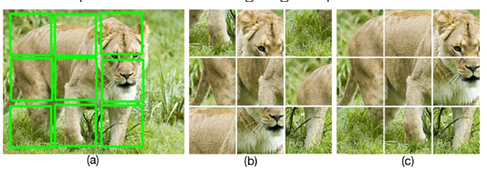
\includegraphics[width=0.5\textwidth]{img/SSL/puzzle.png}
                  \caption{Spatial context structure-based pretext tasks.}
                  \label{fig:SCS}
            \end{figure}

            To limit the number of permutations, usually, Hamming distance is 
            employed to choose only a subset of permutations among all the 
            permutations, i.e., those with a relative large Hamming distance. 
            Only the selected permutations are used to train CNN to recognize the 
            permutation of shuffled image patches.
      \item \textbf{Temporal Context Structure}: The temporal order from videos
            is used as supervision signal. The CNN is trained to verify whether
            the input frame sequence in correct order, or to recognize the order
            of the frame sequence.
\end{itemize}

Features are learned by CNN through the process of solving the pretext tasks
designed based on attributes of the context of images.

\subsection{Free semantic label-based pretext tasks}
This type of pretext tasks train networks with automatically generated semantic
labels. Generally, the free semantic labels such as segmentation masks, depth
images, optical flows, and surface normal images can be rendered by game engine
or generated by hard-code methods.

Since these semantic labels are automatically generated, the methods using the
synthetic datasets or using them in conjunction with a large unlabeled image or
video datasets are considered as self-supervised learning methods.

\begin{note}
      Strictly speaking, the methods based on data generated by game engines
      do/should not belong to the self-supervised learning methods since human
      intervention is needed during the data generation process. However, some
      recent work treat them as self-supervised learning methods.
\end{note}

Game engines can generate realistic images with accurate pixel-level labels with
very low cost. However, due to the domain gap between synthetic and real-world
images, the CNNs purely trained on synthetic images cannot be directly applied
to real-world images. To utilize synthetic datasets for self-supervised feature
learning, the domain gap needs to be explicitly bridged.

To overcome the problem, unsupervised feature space domain adaptation methods
based on adversarial learning have been proposed. The CNN predicts surface normal,
depth, and instance contour for the synthetic images and a discriminator network
$D$ is employed to minimize the difference of feature space domains between
real-world and synthetic data.

\begin{figure}[!ht]
      \centering
      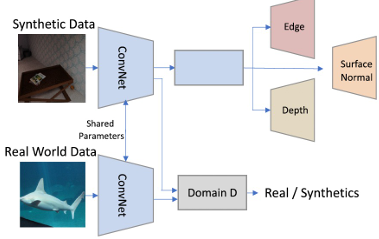
\includegraphics[width=0.5\textwidth]{img/SSL/FreeSemantic.png}
      \caption{Free semantic labels-based pretext tasks.}
      \label{fig:FSL}
\end{figure}

Applying hard-code programs is another way to automatically generate semantic
labels such as salience, foreground masks, contours, depth for images and videos.
With these methods, very large-scale datasets with generated semantic labels can
be used for self-supervised feature learning. This type of methods generally has
two steps:
\begin{enumerate}
      \item Label generation by employing hard-code programs on images or videos
            to obtain labels;
      \item Train CNNs with the generated labels.
\end{enumerate}

No matter what kind of labels used to train CNNs, the general idea of this type
of methods is to distill knowledge from the hard-code detector.

One drawback is that the semantic labels generated by hard-code detector usually
are very noisy which need to be specifically coped with.

\subsection{Cross modal-based pretext tasks}
This type of pretext tasks trains CNNs to verify whether two different channels
of input data are corresponding to each other such as Visual-Audio Correspondence
Verification, RGB-Flow Correspondence Verification, Contrasting (i.e., maximizing
agreement between differently augmented views of the same data example), and egomotion.

\begin{center}
      Egomotion is defined as the 3D motion of a camera within an environment.
      In the field of computer vision, egomotion refers to estimating a camera's
      motion relative to a rigid scene. An example of egomotion estimation would
      be estimating a car's moving position relative to lines on the road or street
      signs being observed from the car itself. The estimation of egomotion is
      important in autonomous robot navigation applications.
\end{center}

Cross modal-based learning methods usually learn features from the correspondence
of multiple data streams.

In addition to rich temporal and spatial information in videos, optical flow
sequence can be generated to specifically indicate the motion in videos, and the
difference of frames can be computed with negligible time and space-time complexity
to indicate the boundary of the moving objects.

Based on the type of data used, these methods fall into three groups:
\begin{itemize}
      \item Methods that learn features by using the RGB and optical flow
            correspondence;
      \item Methods that learn features by utilizing the video and audio correspondence
      \item Ego-motion that learn by utilizing the correspondence between egocentric
            video and egomotorsensor signals.
\end{itemize}

Usually, the network is trained to recognize if the two kinds of input data are
corresponding to each other, or is trained to learn the transformation between
different modalities.
\section{Commonly used downstream tasks for evaluation}
To evaluate the quality of the learned image or video features by self-supervised
methods, the learned parameters by SSL are employed as pre-trained models and then
fine-tuned on downstream tasks such as image classification, semantic segmentation,
object detection, and action recognition etc.

The performance of the transfer learning on these high-level vision tasks
demonstrates the generalizability of the learned features.

If CNNs trained in SSL scenarios can learn general features, then the pre-trained
models can be used as a good starting point for other vision tasks that require
capturing similar features from images or videos.

In addition to the quantitative evaluations of the learned features, there are
also some qualitative visualization methods to evaluate the quality of SSL features.
Three methods are often used for this purpose:
\begin{enumerate}
      \item \textbf{Kernel visualization}: Qualitatively visualize the kernels of
            the first convolution layer learned with the pretext tasks and compare
            the kernels from supervised models. The similarity of the kernels
            learned by supervised and self-supervised models are compared to
            indicate the effectiveness of self supervised methods.
      \item \textbf{Feature Map Visualization}: Feature maps are visualized to
            show the attention of networks. Larger activation represents the neural
            network pays more attention to the corresponding region in the image.
            Feature maps are usually qualitatively visualized and compared with
            that of supervised models.
      \item \textbf{Nearest Neighbor Retrieval}: In general, images with similar
            appearance usually are closer in the feature space. The nearest
            neighbor method is used to find the top $K$ nearest neighbors from
            the feature space of the features learned by the self-supervised
            learned model.
\end{enumerate}
\chapter{Introduction to Explainable AI}
The term \textbf{Explainable AI} (XAI) has been defined in various ways throughout
the literature. In this chapter, we provide an overview of the most common
definitions and concepts. Additionally, we discuss the significance of XAI and
the motivation driving its development.

To begin, let us clarify what XAI is not. \textbf{Explainable AI does not imply
    causality.} Providing an explanation does not necessarily mean the model has
identified a cause-and-effect relationship. AI models typically identify patterns
in data rather than causal links. Therefore, even if a feature is identified as
important to a prediction, it does not imply that the feature caused the observed
outcome.

Explanations in AI can be influenced by human biases and the subjective choice
of explanation methods. Different explainability techniques may produce varying
explanations for the same prediction, potentially leading to inconsistencies.
Furthermore, explanations can be affected by hidden biases in the training data
or the model's underlying logic.

It is important to note that an explanation is not the same as rigorous proof or
scientific validation. Explaining a model's behavior does not equate to formally
verifying its reasoning. A model's reasoning may sound convincing but still be
flawed, as explanations can sometimes rely on spurious correlations or logically
unsound premises, even if they appear coherent.

Despite these limitations, explainability is crucial for building trust in AI
systems. We can define XAI as methods and models that make the behavior and
predictions of machine learning (ML) systems understandable to humans. This is
important for several reasons:

\begin{itemize}
    \item \textbf{Trust}: Users are more likely to trust understandable models,
          particularly in high-stakes applications;
    \item \textbf{Debugging}: Enables users to inspect the patterns discovered
          by AI models and identify potential issues;
    \item \textbf{Fairness}: Helps ensure that the learned relationships are not
          influenced by human biases;
    \item \textbf{Informativeness}: Facilitates the transfer of knowledge from ML
          models to humans;
    \item \textbf{Legal compliance}: Addresses requirements set by regulations
          such as GDPR and the AI Act.
\end{itemize}

\section{Taxonomy of XAI Methods}

There is no single way to categorize XAI methods. Here, we introduce a taxonomy
based on four dimensions:

\subsection{Framework}
\begin{itemize}
    \item \textbf{Interpretable models}: Models that are inherently interpretable,
          such as linear regression or decision trees;
    \item \textbf{Explainability algorithms}: Techniques designed to explain the
          predictions of existing black-box models.
\end{itemize}

\subsection{Scope}
\begin{itemize}
    \item \textbf{Global}: Explains the model's behavior across the entire dataset;
    \item \textbf{Local}: Explains the model's behavior for a specific prediction.
\end{itemize}

\subsection{Applicability}
\begin{itemize}
    \item \textbf{Model-specific}: Explanations tailored to a specific model type;
    \item \textbf{Model-agnostic}: Explanations that are applicable to any model type.
\end{itemize}

\subsection{Produced Results}
\begin{itemize}
    \item \textbf{Feature importance}: Highlights the contribution of each feature
          to the model's predictions;
    \item \textbf{Counterfactual explanations}: Explains how input changes would
          alter the output;
    \item \textbf{Concepts}: Provides explanations in terms of human-friendly
          concepts or abstractions rather than input features;
    \item Additional techniques as applicable.
\end{itemize}

\section{SHAP}
\textbf{SHAP} (SHapley Additive exPlanations) is a unified approach to explain
the outputs of machine learning models. It is based on cooperative game theory,
which studies interactions between rational agents. In this context, the "agents"
are the features of the input data, and the goal is to predict the model's output.

SHAP values are derived from the Shapley value, a concept from cooperative game
theory. SHAP computes all possible coalitions of features and evaluates the
contribution of each feature to the prediction using a utility function. This
\textit{utility function} represents the total value the coalition achieves by
working together. The Shapley values provide a fair distribution of this value
among the features in the coalition.

\section{LIME}
\textbf{LIME} (Local Interpretable Model-agnostic Explanations) is a model-agnostic
technique for explaining predictions made by machine learning models. LIME works
by approximating the decision boundary of the original model locally, around a
specific prediction. It creates a simpler and interpretable surrogate model that
approximates the behavior of the complex model in the neighborhood of the given
prediction.
\end{document}